% !TEX program = pdflatex
% Compile from docs/ so that relative paths to ../src/ resolve.
\documentclass[11pt]{article}

% =============================================================================
% Layout
% =============================================================================
\usepackage[margin=1in]{geometry}
\usepackage{microtype}
\usepackage{parskip}
\setlength{\emergencystretch}{3em}
\usepackage{float}
\usepackage{tikz}
\usetikzlibrary{arrows.meta, positioning, calc, fit, backgrounds,
                decorations.pathreplacing, shapes.geometric}

% =============================================================================
% Fonts (Computer Modern via Latin Modern, default LaTeX look)
% =============================================================================
\usepackage[T1]{fontenc}
\usepackage{lmodern}
\usepackage[scaled=0.92]{inconsolata}

% =============================================================================
% Math
% =============================================================================
\usepackage{amsmath}
\usepackage{amssymb}

% =============================================================================
% Graphics, tables
% =============================================================================
\usepackage{graphicx}
\usepackage{grffile}            % allow special characters in image filenames
\usepackage{xcolor}
\usepackage{booktabs}
\usepackage{array}
\usepackage{multirow}
\usepackage{longtable}
\usepackage{caption}
\usepackage{subcaption}

% =============================================================================
% Callouts and code
% =============================================================================
\usepackage[most]{tcolorbox}
\usepackage{listings}

% =============================================================================
% Hyperlinks
% =============================================================================
\usepackage{hyperref}

% =============================================================================
% Colour palette (shared by every section)
% =============================================================================
\definecolor{accent}{HTML}{2E5A88}        % deep blue
\definecolor{accentred}{HTML}{C44E52}     % warm red diagram highlights
\definecolor{accentgreen}{HTML}{3F8F5F}   % green for "same author" / TP
\definecolor{softgray}{HTML}{F5F5F7}      % callout background
\definecolor{rule}{HTML}{B7C2D0}          % thin separator
\definecolor{codebg}{HTML}{F2F4F7}        % inline code background

% =============================================================================
% Section formatting (standard black LaTeX style)
% =============================================================================
\usepackage{titlesec}
\titleformat{\section}{\Large\bfseries}{\thesection}{0.6em}{}
\titleformat{\subsection}{\large\bfseries}{\thesubsection}{0.5em}{}
\titleformat{\subsubsection}{\normalsize\bfseries}{\thesubsubsection}{0.4em}{}
\titlespacing*{\section}{0pt}{1.4em}{0.6em}

% =============================================================================
% Caption styling
% =============================================================================
\captionsetup{font=small, labelfont=bf, skip=4pt}

% =============================================================================
% Hyperref styling (subtle black links)
% =============================================================================
\hypersetup{colorlinks=true, linkcolor=black, urlcolor=black, citecolor=black,
            hypertexnames=false}

% =============================================================================
% Inline code chip
% =============================================================================
\newcommand{\code}[1]{%
  \tcbox[on line, colback=codebg, colframe=codebg,
         boxrule=0pt, arc=2pt, left=2pt, right=2pt, top=0pt, bottom=0pt]
        {\ttfamily\small #1}}

% =============================================================================
% Shell listing style
% =============================================================================
\lstdefinestyle{shell}{
  basicstyle=\ttfamily\small,
  backgroundcolor=\color{codebg},
  frame=single, framerule=0.4pt, rulecolor=\color{rule},
  xleftmargin=6pt, xrightmargin=6pt, framexleftmargin=6pt,
  breaklines=true, columns=fullflexible, keepspaces=true,
  showstringspaces=false, aboveskip=6pt, belowskip=6pt,
  commentstyle=\color{accent}, morecomment=[l]{\#},
}

% =============================================================================
% Callout box
% =============================================================================
\newtcolorbox{keybox}{
  enhanced, breakable,
  colback=white, colframe=black,
  boxrule=0.4pt, arc=4pt,
  left=10pt, right=10pt, top=6pt, bottom=7pt,
  before skip=10pt, after skip=10pt,
}
\newcommand{\keytitle}[1]{\noindent\textbf{#1}\enspace\ignorespaces}

% =============================================================================
% Title block (PDF metadata only — cover page is built explicitly below)
% =============================================================================
\title{Authorship Identification via Writing Style: A Case Study on LessWrong}
\author{Group 4 --- SoICT, HUST}
\date{June 10, 2026}

\begin{document}

% =============================================================================
% Cover page
% =============================================================================
\begin{titlepage}
\centering
\vspace*{0.2cm}

% Institutional header (\Large so the long HUST line stays on one line)
{\Large\bfseries HANOI UNIVERSITY OF SCIENCE AND TECHNOLOGY\par}
\vspace{0.45em}
{\large School of Information and Communications Technology\par}

\vspace{0.55cm}
\rule{0.82\linewidth}{0.6pt}

\vspace{0.7cm}
% Logo

\includegraphics[width=0.28\linewidth]{logo.png}

\vspace{0.8cm}
% Title
{\Huge\bfseries Authorship Identification\\[0.15em]via Writing Style\par}
\vspace{0.6em}
{\Large\itshape A Case Study on LessWrong\par}

\vspace{0.5cm}
\rule{0.55\linewidth}{0.4pt}

\vspace{0.8cm}
% Course and instructor
{\Large\textbf{Course:}\enspace Machine Learning (IT3190E)\par}
\vspace{0.35em}
{\Large\textbf{Instructor:}\enspace Associate Professor Than Quang Khoat\par}

\vspace{0.8cm}
% Group block
{\LARGE\bfseries Group 4\par}
\vspace{0.5em}
\renewcommand{\arraystretch}{1.18}
{\large
\begin{tabular}{@{}l@{\hspace{3em}}r@{}}
  Nguy\~{\^e}n L\^e Anh                & 202416663 \\
  L\^e Xu\^an Nh\d{\^a}t Kh\^oi         & 202416711 \\
  Tr\`{\^a}n M\d{a}nh To\`an            & 202416753 \\
  \DJ\d{\u a}ng Ho\`ang Vi\d{\^e}t      & 202416765 \\
  B\`ui Nguy\^en V\~u                   & 202416768 \\
  Ph\d{a}m Quang V\~u                   & 202416767 \\
\end{tabular}
\par}

\vfill
{\Large\itshape Hanoi, June 10, 2026\par}
\vspace*{0.3cm}
\end{titlepage}

\begin{abstract}
\noindent We study \textbf{authorship stylometry} on long-form essays drawn from the
LessWrong platform. From a single crawling pipeline we build three custom
sub-datasets, each shaped to fit a different downstream task, and ask three
questions of growing difficulty.
\textit{First}, can an unsupervised method recover author identity from style alone?
We use \textbf{K-means} on $107$ stylometric features and trace how clustering
quality depends on the number of authors, articles per author, article length,
and the era in which a piece was written. \textit{Second}, can a supervised model
decide whether two previously unseen articles share an author? We frame this as
binary same-author detection with a \textbf{Support Vector Machine} on engineered
pair features, and compare it against a \textbf{Logistic Regression} baseline.
\textit{Third}, can a model identify the author of a article from a closed set,
while also refusing to attribute work to anyone outside that set? We train a
small \textbf{neural network} as a six-way classifier that includes an explicit
``none-of-the-above'' class. Each method tells a slightly different story about
the same underlying signal --- and together they show that stylistic identity in
long-form essays is strong, mostly linearly accessible, and remarkably stable
once a few practical pitfalls are handled.
\end{abstract}

\vspace{0.8em}
{\setcounter{tocdepth}{2}\small\tableofcontents}
\clearpage

% =============================================================================
\section{Introduction}
\label{sec:intro}

Two people writing about the same topic make a thousand tiny choices that have
nothing to do with the topic itself --- how often they reach for a semicolon,
whether they prefer ``which'' or ``that'', how long they let a sentence run, how
often they hedge with ``perhaps'' or ``arguably'', what fraction of their words
come from the closed list of English function words. The premise of stylometry
is that those choices, taken together, leave a fingerprint that is far more
characteristic of the writer than of the writing.

This project tests that premise on a single corpus --- long-form essays from
LessWrong --- using three families of method that approach the same question
from increasingly committed angles:

\begin{itemize}\setlength\itemsep{2pt}
  \item \textbf{Unsupervised (K-means).} Given a pile of articles by $K$
        unknown authors, can a clustering algorithm recover the author groups
        using nothing but writing style?
  \item \textbf{Supervised pairwise (SVM, Logistic Regression).} Given two
        articles by authors the model has never seen, can a classifier decide
        whether they were written by the same person?
  \item \textbf{Supervised identification (Neural Network).} Given a article
        from one of five known authors --- or possibly from someone outside the
        list entirely --- can a network name the author or correctly decline?
\end{itemize}

The four sections below mirror this progression. Section~\ref{sec:data} describes
how the corpus was crawled and cleaned, including the three sub-datasets that
later sections draw from. Section~\ref{sec:kmeans} runs K-means, isolates the
effects of dataset density and writing era, and uses the law of large numbers to
explain a striking length-saturation effect. Section~\ref{sec:svm} reframes the
task as pairwise verification, builds an SVM with an RBF kernel, and contrasts
it with a linear logistic-regression baseline. Section~\ref{sec:nn} closes the
loop with a small neural network that classifies among five known authors plus
an explicit unknown-author class, and uses a gradient-health diagnostic to
explain why deeper architectures collapse on this kind of tabular feature.

% =============================================================================
\section{Building the Dataset}
\label{sec:data}

The first practical question is where the data comes from. LessWrong is a
long-running essayistic forum whose posts are, on the whole, longer and more
deliberately written than most blog content --- exactly the regime in which
stylometric features stand a chance of converging. The platform also exposes a
public GraphQL API, which makes high-volume but well-targeted crawling
straightforward.

\subsection{What we want to collect}

We chose to assemble \emph{three} sub-datasets in parallel rather than one large
generic one. Each sub-dataset is tailored to a downstream question, and that
specialisation matters: an experiment about era effects, for instance, requires
each author to have a controlled number of articles on either side of a cutoff
year, which a generic corpus would not guarantee. The three sub-datasets are:

\begin{itemize}\setlength\itemsep{3pt}
  \item \textbf{\texttt{cleaned\_5}} --- five high-volume authors with up to
        $150$ articles each, split as exactly $5$ articles from
        $\geq 2025$ and up to $145$ from $\leq 2024$. This is the
        ``deep'' dataset used by the neural-network section for the five
        known authors.
  \item \textbf{\texttt{cleaned\_10}} --- ten authors with a strict
        $20$-articles-from-$\leq 2022$ and $20$-articles-from-$\geq 2024$
        split per author. Articles from 2023 are excluded so the two eras are
        cleanly separated by the rise of public LLM chatbots. This is the
        corpus used in the K-means era experiment and in most of its sweep
        experiments.
  \item \textbf{\texttt{cleaned\_35}} --- the breadth dataset, $35$ authors
        with between $30$ and $50$ articles each (no time constraints). This is
        the pool the K-means \emph{number-of-authors} sweep draws from, and the
        same pool the SVM treats as a $1{,}484$-article corpus.
\end{itemize}

Throughout, an ``article'' means a single LessWrong post of at least $1{,}500$
words after cleaning. The length floor exists because, as Section~\ref{sec:kmeans}
will show, most stylometric features need on the order of a thousand words to
stabilise around their author-specific means.

\subsection{Crawling}

The crawl is driven by three Python scripts, one per sub-dataset, each issuing
POST requests against LessWrong's GraphQL endpoint. They share a small
infrastructure stack:

\begin{itemize}\setlength\itemsep{1pt}
  \item \code{requests} sends the GraphQL queries, paginates over an author's
        posts, and handles transient failures.
  \item \code{BeautifulSoup} parses the returned \texttt{htmlBody}, strips
        structural noise (\texttt{<img>}, \texttt{<figure>}, \texttt{<script>},
        and similar non-textual blocks), and unwraps hyperlinks to retain the
        anchor text only.
  \item \code{re} enforces the length floor via the token pattern
        \verb|\b[\w'-]+\b|, which counts ``don't'' or ``state-of-the-art'' as
        single words rather than splitting on the apostrophe or hyphen.
\end{itemize}

\begin{center}
\begin{minipage}{0.62\textwidth}
\begin{lstlisting}[style=shell]
pip install requests beautifulsoup4
python crawl_lesswrong5.py    # -> raw/raw_5/
python crawl_lesswrong10.py   # -> raw/raw_10/
python crawl_lesswrong35.py   # -> raw/raw_35/
\end{lstlisting}
\end{minipage}
\end{center}

Each script writes one JSON file per author into its dedicated raw output
directory --- \code{dataset/raw/raw\_5/}, \code{dataset/raw/raw\_10/}, and
\code{dataset/raw/raw\_35/} respectively --- with one record per article and
metadata (slug, posted date, word count) attached so later filters and sweeps
can operate without re-reading the body.

\subsection{Cleaning}

GraphQL gives us reasonably clean HTML, but the body of a real LessWrong post
contains plenty of material that should not feed a stylometric feature. The
raw output is therefore passed through a two-stage cleaning step --- automated
followed by manual review --- to remove the following recurring noise:

\begin{itemize}\setlength\itemsep{1pt}
  \item \textbf{Reposting boilerplate.} Articles that begin with notices such
        as \textit{``This post originally appeared on \dots''} or
        \textit{``Crossposted from \dots''}, which pull the style toward the
        original venue rather than the author.
  \item \textbf{Non-prose posts.} Audio transcripts, link-roundup pages, and
        posts dominated by tables, source code, MathJax formulas, or large
        block quotes. Any of these would swamp the rate-based stylometric
        features with material that the author may not have written in their
        own voice at all.
\end{itemize}

After cleaning, articles that no longer meet the $1{,}500$-word floor or are
otherwise unsuitable are dropped from the dataset and recorded in a
\code{\_dropped.jsonl} log so the decision is auditable. The surviving
articles are written to \code{dataset/cleaned/cleaned\_5/},
\code{dataset/cleaned/cleaned\_10/}, and \code{dataset/cleaned/cleaned\_35/},
mirroring the raw directory layout.

\subsection{Final statistics}

The three tables below report the per-author article counts that survive
cleaning. Throughout the rest of the report, these are the numbers each
experiment draws from.

\begin{table}[H]
\centering
\small
\caption{\texttt{cleaned\_5}: deep dataset for the five known authors used by
the neural network. ``$\geq 2025$'' and ``$\leq 2024$'' refer to the
strict $5$/$145$ post-by-year split per author.}
\label{tab:dataset_cleaned_5}
\begin{tabular}{@{}clccc@{}}
\toprule
\textbf{No.} & \textbf{Author (slug)} & \textbf{$\geq 2025$} & \textbf{$\leq 2024$} & \textbf{Total} \\
\midrule
1 & \code{eliezer\_yudkowsky} & 5 & 145 & 150 \\
2 & \code{johnswentworth}     & 5 & 145 & 150 \\
3 & \code{raemon}             & 5 & 121 & 126 \\
4 & \code{scottalexander}     & 2 & 145 & 147 \\
5 & \code{zvi}                & 5 & 145 & 150 \\
\midrule
\multicolumn{2}{l}{\textbf{Total}} & \textbf{22} & \textbf{701} & \textbf{723} \\
\bottomrule
\end{tabular}
\end{table}

\begin{table}[H]
\centering
\small
\caption{\texttt{cleaned\_10}: era-split dataset used by the K-means era
experiment and most of its sweeps. Articles from 2023 are deliberately
excluded to cleanly separate the pre-chatbot and post-chatbot eras.}
\label{tab:dataset_c10}
\begin{tabular}{@{}clccc@{}}
\toprule
\textbf{No.} & \textbf{Author (slug)} & \textbf{$\geq 2024$} & \textbf{$\leq 2022$} & \textbf{Total} \\
\midrule
1  & \code{abramdemski}        & 20 & 20 & 40 \\
2  & \code{jessica-liu-taylor} & 20 & 20 & 40 \\
3  & \code{johnswentworth}     & 20 & 20 & 40 \\
4  & \code{kaj\_sotala}        & 20 & 20 & 40 \\
5  & \code{neel-nanda-1}       & 20 & 20 & 40 \\
6  & \code{raemon}             & 20 & 20 & 40 \\
7  & \code{ricraz}             & 20 & 20 & 40 \\
8  & \code{ruby}               & 20 & 20 & 40 \\
9  & \code{steve2152}          & 20 & 20 & 40 \\
10 & \code{zvi}                & 20 & 20 & 40 \\
\midrule
\multicolumn{2}{l}{\textbf{Total}} & \textbf{200} & \textbf{200} & \textbf{400} \\
\bottomrule
\end{tabular}
\end{table}

\begin{table}[H]
\centering
\small
\caption{\texttt{cleaned\_35}: breadth dataset used by the K-means
number-of-authors sweep and the SVM verification experiment.}
\label{tab:dataset_c35}
\begin{tabular}{@{}l r @{\hspace{3em}} l r @{\hspace{3em}} l r@{}}
\toprule
\textbf{Author} & \textbf{\#} & \textbf{Author} & \textbf{\#} & \textbf{Author} & \textbf{\#} \\
\midrule
\code{david-gross}            & 50 & \code{ryan\_greenblatt}    & 44 & \code{lukeprog}        & 38 \\
\code{screwtape}              & 49 & \code{jasoncrawford}       & 44 & \code{elizabeth-1}     & 36 \\
\code{scottalexander}         & 49 & \code{raemon}              & 43 & \code{benito}          & 34 \\
\code{sarahconstantin}        & 49 & \code{buck}                & 42 & \code{turntrout}       & 33 \\
\code{steve2152}              & 48 & \code{joe-carlsmith}       & 42 & \code{philh}           & 29 \\
\code{adamshimi}              & 48 & \code{ruby}                & 42 & \code{jan\_kulveit}    & 27 \\
\code{kaj\_sotala}            & 48 & \code{zack\_m\_davis}      & 41 & \code{nunosempere}     & 27 \\
\code{ricraz}                 & 47 & \code{so8res}              & 40 & & \\
\code{zvi}                    & 47 & \code{petermccluskey}      & 40 & & \\
\code{jessica-liu-taylor}     & 47 & \code{jacob-falkovich}     & 39 & & \\
\code{katjagrace}             & 47 & \code{holdenkarnofsky}     & 38 & & \\
\code{tsvibt}                 & 47 & & & & \\
\code{benquo}                 & 46 & & & & \\
\code{eliezer\_yudkowsky}     & 46 & & & & \\
\code{johnswentworth}         & 46 & & & & \\
\code{gordon-seidoh-worley}   & 46 & & & & \\
\code{abramdemski}            & 45 & & & & \\
\midrule
\multicolumn{6}{r}{\textbf{Total: 1{,}484 articles across 35 authors}} \\
\bottomrule
\end{tabular}
\end{table}

% =============================================================================
\section{Unsupervised Clustering with K-means}
\label{sec:kmeans}

\textit{Given a set of articles written by $K$ authors, how well can we recover
the author groups using only writing style? Perhaps the most natural algorithm
to study this question is K-means.}

\subsection{Clustering 10 Authors}

\paragraph{Dataset and preprocessing.}
We use the \texttt{cleaned\_10} corpus: 10 authors, 40 articles each, evenly
split across two periods (20 from $\leq 2022$, 20 from $\geq 2024$). To keep
article length from masking the stylistic signal, we truncate every article to
its first \textbf{1{,}500 words} and discard anything past the cutoff.

\paragraph{Feature extraction.}
We extract \textbf{107} known stylometric features per article using
\code{NLTK} for tokenisation and POS-tagging. The features fall into seven
groups:
\begin{itemize}\setlength\itemsep{1pt}
  \item \textbf{Word and sentence length} statistics (mean, standard deviation,
        median, fractions of 1--6 character words, etc.)
  \item \textbf{Vocabulary richness}: type-token ratio, hapax ratio, Yule~$K$,
        Simpson~$D$, Brun\'et~$W$, Honor\'e~$R$
  \item \textbf{Function-word frequencies}: usage rate of each of the top-50
        English function words (``the'', ``and'', ``I'', ``you'', \ldots)
  \item \textbf{Stylistic word categories}: rates for hedges, amplifiers,
        discourse markers, and conjunctions
  \item \textbf{Punctuation rates}: commas, periods, semicolons, parentheses, etc.
  \item \textbf{Coarse POS-tag distributions}: noun, verb, adjective, adverb,
        pronoun, determiner, preposition, conjunction, modal fractions
  \item \textbf{Character-level ratios}: uppercase fraction, vowel frequencies
\end{itemize}
Features with zero variance across the corpus are dropped; the rest are
z-scored with \code{sklearn}'s \code{StandardScaler} so every feature has mean
0 and standard deviation 1 before clustering.

\paragraph{Clustering.}
We run \code{sklearn.cluster.KMeans} with $K=10$, \code{init="k-means++"}, and
\code{n\_init=10}: the algorithm makes ten independent attempts and returns the
one with the lowest \textbf{within-cluster sum of squares}, the
\emph{distortion}
\[
  L \;=\; \sum_{k=1}^{K} \sum_{\mathbf{x} \in C_k}
          \lVert \mathbf{x} - \boldsymbol{\mu}_k \rVert^2,
\]
where $C_k$ is the set of articles assigned to cluster $k$ and
$\boldsymbol{\mu}_k$ is its centroid.

\paragraph{Measuring performance: the Adjusted Rand Index.}
A natural measure of clustering quality compares the cluster assignments
against the true author labels by examining every \emph{pair} of articles. For a
dataset of $n$ articles there are $\binom{n}{2}$ such pairs. For each pair, the
clustering either \textbf{agrees} with the ground truth (both labellings put
the two articles in the same group, or both put them in different groups) or it
\textbf{disagrees}. The \textbf{Rand Index (RI)} is simply the fraction of pairs
on which the clustering agrees:
\[
  \mathrm{RI}
  = \frac{\text{number of agreeing pairs}}{\displaystyle\binom{n}{2}}.
\]
The problem is that even a random clustering achieves a high RI. With ten
authors and $400$ articles most pairs are from different authors; a random
partition will still separate them most of the time, racking up agreements for
free. The \textbf{Adjusted Rand Index (ARI)} subtracts the agreement expected
from a random partition, rescaling so that random chance scores exactly $0$:
\begin{itemize}\setlength\itemsep{1pt}
  \item \textbf{ARI $= 1$}: perfect recovery of the true author groups.
  \item \textbf{ARI $\approx 0$}: no better than random chance.
  \item \textbf{ARI $< 0$}: systematically worse than random.
\end{itemize}
It is worth noting that ARI depends only on which pairs of points are grouped
together or separated, not on the labels assigned to the clusters.

\paragraph{Results.}
The $400$-article input matrix is $400 \times 107$ after feature extraction.

\begin{figure}[H]
  \centering
  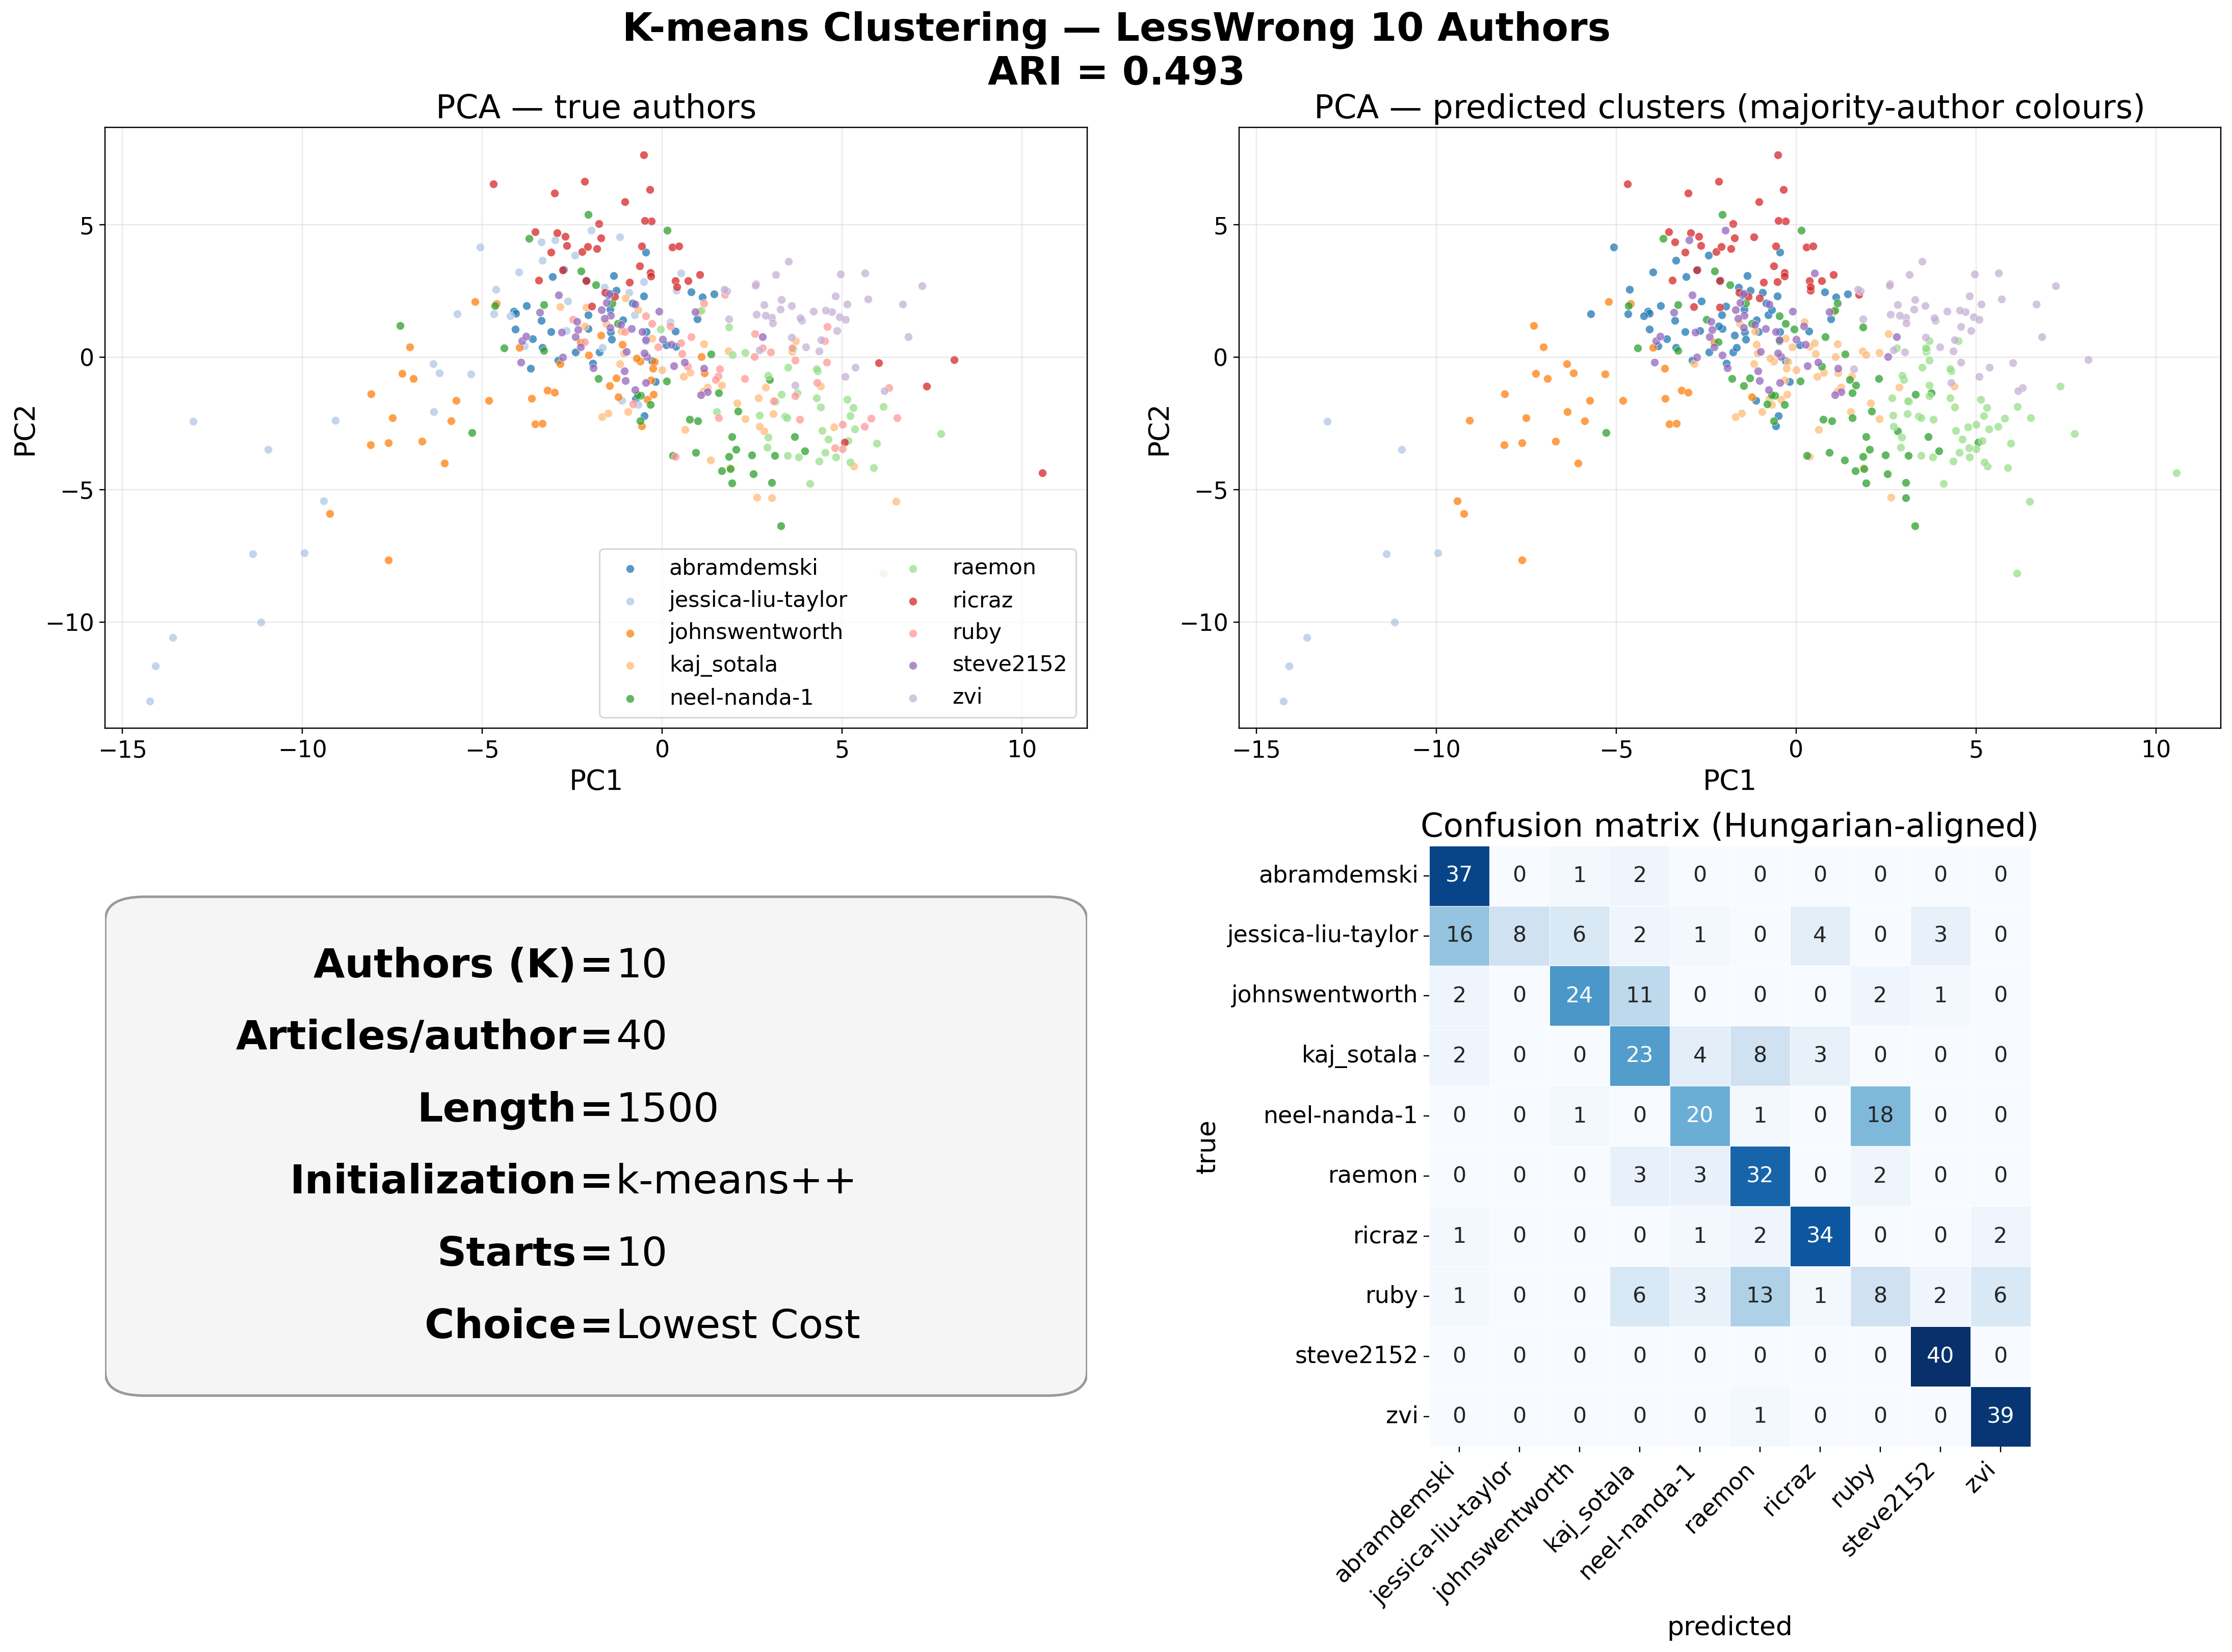
\includegraphics[width=0.82\linewidth]{../src/kmeans/outputs/cluster_10/clustering.png}
  \caption{K-means on the \texttt{cleaned\_10} dataset, $K=10$. \textit{Top
  left}: articles projected onto the two PCA directions of largest variance
  (\code{sklearn.decomposition.PCA} applied to the centered, z-scored matrix),
  coloured by true author. \textit{Top right}: same projection, coloured by
  predicted cluster (each cluster takes the colour of its majority author).
  \textit{Bottom right}: confusion matrix after a Hungarian one-to-one
  alignment (\code{scipy.optimize.linear\_sum\_assignment}) between predicted
  clusters and true authors.}
  \label{fig:cluster10}
\end{figure}

The clustering achieves \textbf{ARI $= 0.49$}, which is fairly impressive given
that we are trying to separate ten groups simultaneously. The confusion matrix
shows a prominent diagonal: most authors land mostly in their own cluster.

Despite this strong result, a question remains: if we were to run the exact
same experiment again, would we still see a similar ARI? K-means is a
randomised algorithm. To cluster the articles, it must first place $K$ initial
centroids somewhere in the feature space. Different starting positions lead to
different final clusters, and the algorithm can get stuck in different local
minima of $L$. \textbf{k-means++} is a smarter initialisation strategy than
placing centroids uniformly at random: it places each subsequent centroid with
probability proportional to its squared distance from the nearest centroid
already chosen, biasing the starting configuration toward spread-out positions
and improving convergence. But k-means++ is still random.

The randomness is controlled by a single integer called the \emph{master seed}
(\code{random\_state} in sklearn). Given a seed, sklearn generates a fully
deterministic sequence of random numbers. For each of the \code{n\_init=10}
attempts, k-means++ draws the next values from this sequence to select $K$
starting centroids. The ten attempts therefore use different starting centroids
(drawn sequentially from the same seed's stream), each converges independently
to some local minimum, and each records its own distortion $L_i$. sklearn
returns the attempt $i^* = \arg\min_i L_i$ with the lowest distortion, for
which ARI is calculated.

The key issue is that all ten attempts are tied to one seed. Change the seed,
and sklearn generates a different random-number sequence, produces a different
pool of ten starting configurations, and may return a different ``best''
clustering with a different ARI. With \code{random\_state=42} we obtained
ARI $= 0.49$, but without running other seeds we cannot tell whether this is
a typical outcome or a lucky one. To measure the variability, we treat each
seed as an independent trial: for ten seed values $(42, 100, 200, \ldots, 900)$
we run the same experiment and record the ARI of the lowest-distortion attempt.
Figure~\ref{fig:seed_diagram} illustrates the procedure.

\begin{figure}[H]
\centering
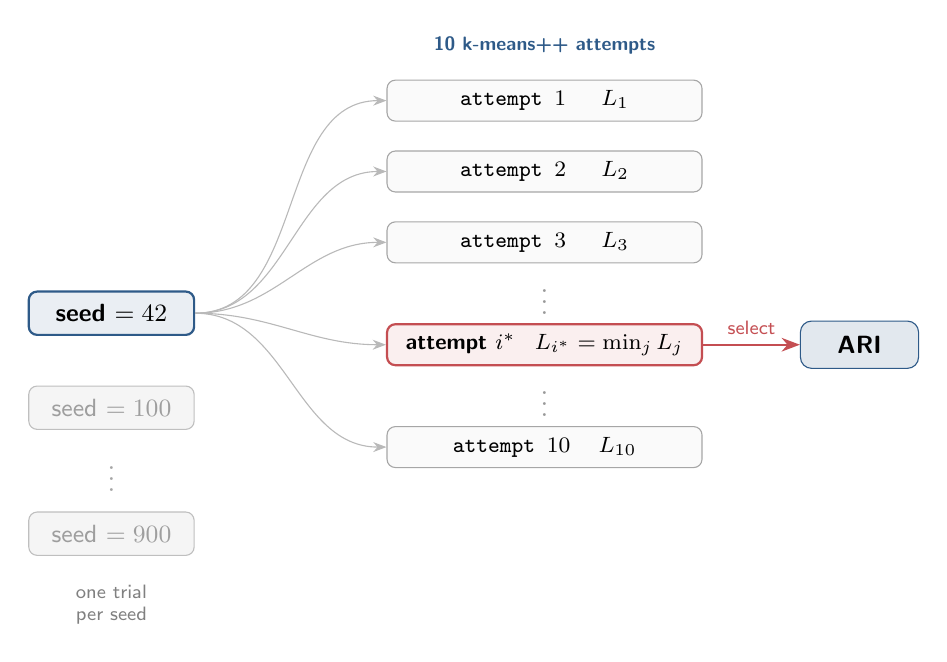
\begin{tikzpicture}[
  seedbox/.style={
    draw=accent, fill=accent!10, rounded corners=3pt,
    minimum width=2.1cm, minimum height=0.55cm,
    align=center, font=\small\sffamily\bfseries, thick
  },
  fadedseed/.style={
    draw=black!25, fill=black!4, rounded corners=3pt,
    minimum width=2.1cm, minimum height=0.55cm,
    align=center, font=\small\sffamily, text=black!38
  },
  trybox/.style={
    draw=black!35, fill=gray!4, rounded corners=3pt,
    minimum width=4.0cm, minimum height=0.52cm,
    align=center, font=\footnotesize\ttfamily
  },
  bestbox/.style={
    draw=accentred, fill=accentred!9, rounded corners=3pt,
    minimum width=4.0cm, minimum height=0.52cm,
    align=center, font=\footnotesize\sffamily\bfseries, thick
  },
  aribox/.style={
    draw=accent, fill=accent!14, rounded corners=4pt,
    minimum width=1.5cm, minimum height=0.6cm,
    align=center, font=\small\sffamily\bfseries
  },
  garr/.style={->, >=Stealth, gray!55, thin},
  barr/.style={->, >=Stealth, accentred, thick},
]
\node[seedbox]   (s42)  at (0,  2.8) {seed $= 42$};
\node[fadedseed] (s100) at (0,  1.6) {seed $= 100$};
\node[text=black!35, font=\normalsize] at (0, 0.8) {$\vdots$};
\node[fadedseed] (s900) at (0,  0.0) {seed $= 900$};
\node[font=\scriptsize\sffamily, text=black!50, align=center]
  at (0, -0.9) {one trial\\per seed};
\node[font=\scriptsize\sffamily\bfseries, text=accent, align=center]
  at (5.5, 6.2) {10 k-means++ attempts};
\node[trybox]  (a1)    at (5.5, 5.5) {attempt $1$\hspace{1.5em}$L_1$};
\node[trybox]  (a2)    at (5.5, 4.6) {attempt $2$\hspace{1.5em}$L_2$};
\node[trybox]  (a3)    at (5.5, 3.7) {attempt $3$\hspace{1.5em}$L_3$};
\node[text=black!40, font=\normalsize] at (5.5, 3.05) {$\vdots$};
\node[bestbox] (abest) at (5.5, 2.4)
  {attempt $i^*$\hspace{0.8em}$L_{i^*} = \min\nolimits_j L_j$};
\node[text=black!40, font=\normalsize] at (5.5, 1.75) {$\vdots$};
\node[trybox]  (a10)   at (5.5, 1.1) {attempt $10$\hspace{1.2em}$L_{10}$};
\foreach \a in {a1,a2,a3,abest,a10} {
  \draw[garr] (s42.east) to[out=0, in=180] (\a.west);
}
\node[aribox] (ari) at (9.5, 2.4) {ARI};
\draw[barr] (abest.east) -- node[above, font=\scriptsize\sffamily]{select} (ari.west);
\end{tikzpicture}
\caption{Procedure for one stability trial. The master seed generates a
deterministic random-number sequence; k-means++ draws from it to produce ten
independent starting configurations. Each attempt converges to a local minimum
of $L$, and the one with the lowest distortion $L_{i^*}$ is selected and scored
with ARI. Running ten different seeds gives ten independent ARI measurements.}
\label{fig:seed_diagram}
\end{figure}

\begin{figure}[H]
  \centering
  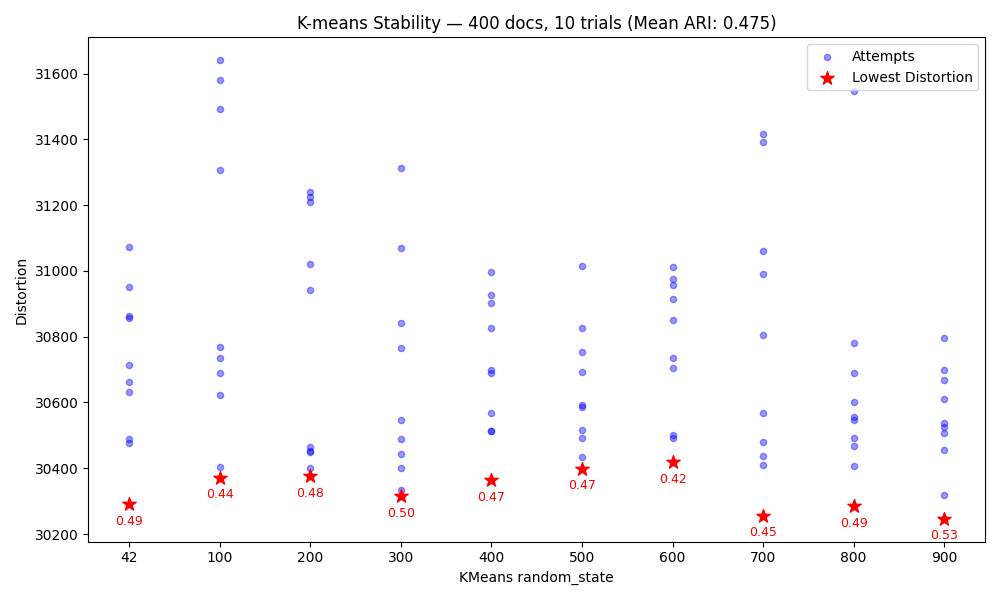
\includegraphics[width=0.78\linewidth]{../src/kmeans/outputs/cluster_10/ari_vs_seed.png}
  \caption{ARI of the selected attempt (lowest $L$) across ten master seeds.
  Blue dots show the distortions of all ten attempts within each trial; the
  red star marks the one sklearn returns. The annotated value is that run's ARI.}
  \label{fig:seed_stability}
\end{figure}

Across the ten trials the mean ARI is \textbf{$0.475$}, ranging from
\textbf{$0.42$} to \textbf{$0.53$}. Our initial result of $0.49$ sits close to
the mean.

\subsection{\texorpdfstring{Effect of Articles per Author ($M$)}{Effect of Articles per Author (M)}}

How does data density, represented by the number of articles per author $M$,
affect performance? An author's writing style varies between articles, often
substantially: they may write across multiple topics and genres, each dragging
the surface features in different directions. An opinion piece tends to use
the word ``I'' more often than a report, for example, and the rate of ``I'' is
one of our features. LessWrong articles also carry residual noise from code
blocks, MathJax formulas, image captions, quoted material, and audio
transcripts that are difficult to remove perfectly. With too few articles per
author, the sample likely becomes a poor estimate of that author's true style,
so we expect K-means performance to degrade as $M$ shrinks.

\paragraph{Setup.}
We reuse the \texttt{cleaned\_10} corpus, fix $K=4$ and length
$N=1{,}500$ words, and sweep $M \in \{5, 10, 15, 20\}$. For each $M$ we run
$50$ trials: sample $4$ of the $10$ authors at random, sample $M$ articles per
author, truncate each at the first $N$ words, extract features, cluster with
$10$ k-means++ initialisations, select the attempt with the lowest distortion,
and record ARI.

\begin{figure}[H]
  \centering
  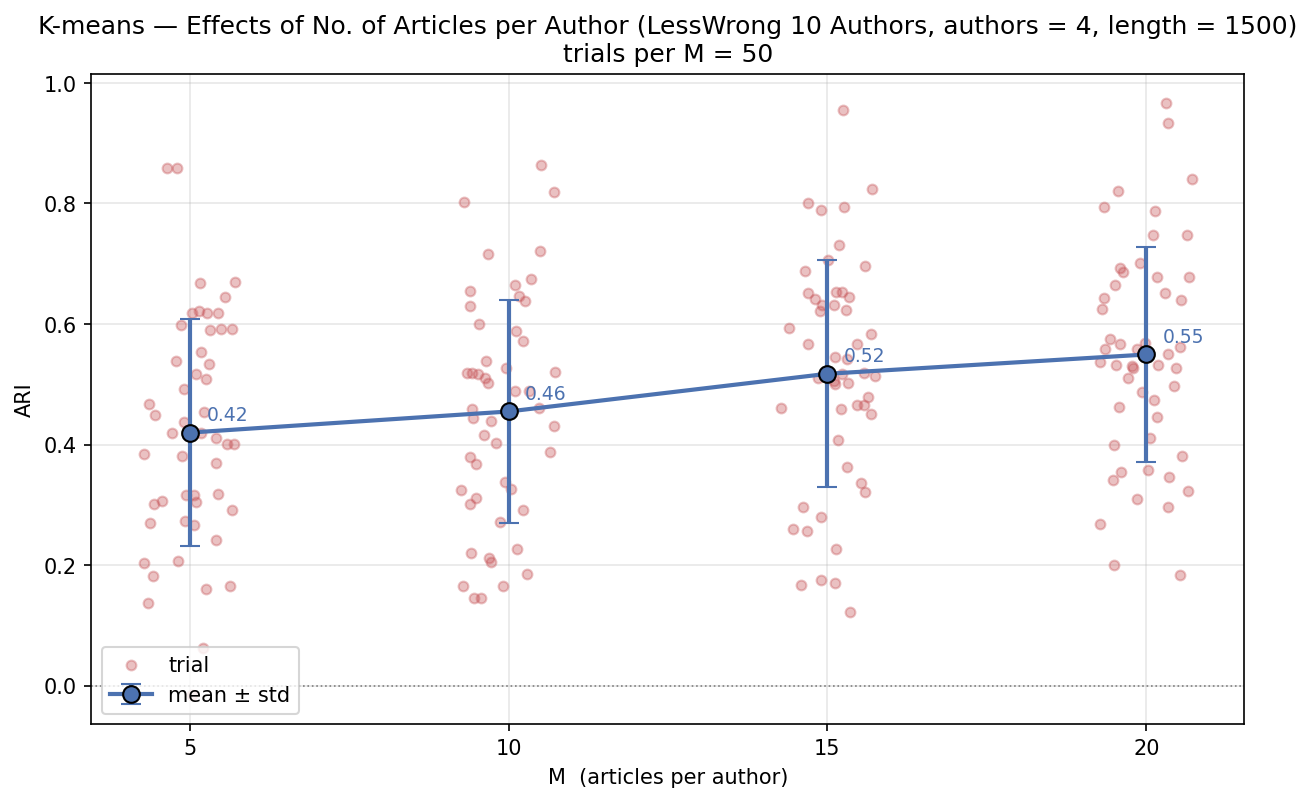
\includegraphics[width=0.82\linewidth]{../src/kmeans/outputs/effect_of_m/ari_vs_m_10authors.png}
  \caption{ARI vs.\ $M$ on \texttt{cleaned\_10} ($K=4$, $N=1500$, $50$ trials
  per $M$). Mean ARI rises from $0.42$ at $M=5$ to $0.55$ at $M=20$.}
  \label{fig:m10}
\end{figure}

ARI rises steadily from $0.42$ at $M=5$ to $0.55$ at $M=20$, with the curve
still climbing at the upper end of the sweep. It is unclear whether performance
would continue to improve past $M=20$ or eventually saturate.

To study higher values of $M$, the number of articles available per author
needs to be considerably larger than the maximum $M$ we intend to sample.
Otherwise, for large $M$, the articles sampled for each author will largely
overlap across trials, so ARI variability will mostly reflect which author
group was sampled rather than which articles. With $4$ authors drawn from $10$,
trials already tend to share authors, so that source of variability is limited
to begin with. Finding $10$ or more LessWrong authors with that many qualifying
articles (length $\geq 1{,}500$ words) turns out to be difficult. We therefore
restrict to a separate \textit{4 Authors} subset, four specific authors for
whom we were able to find $76$--$79$ articles each. While any conclusions will
be specific to these four authors, the results can still hint at whether
collecting more articles per author is worth the effort.

\begin{figure}[H]
  \centering
  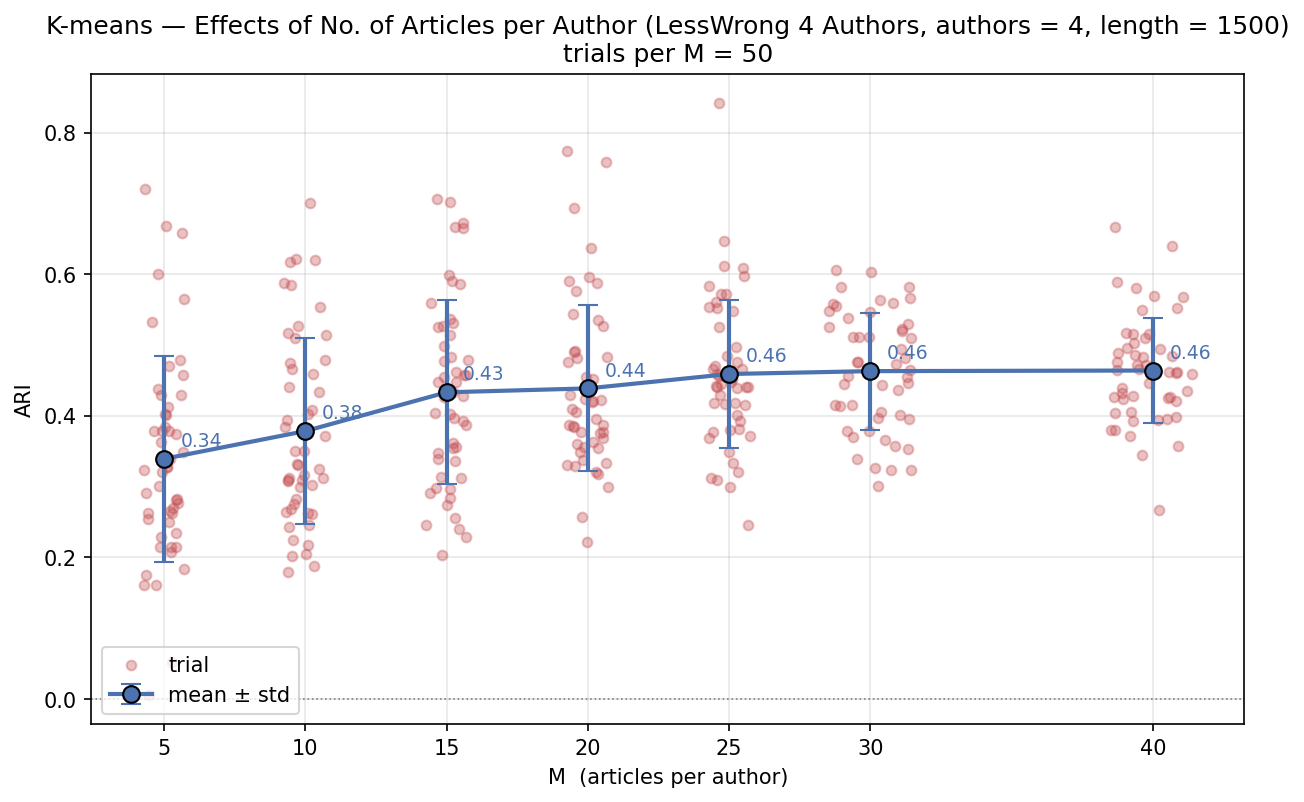
\includegraphics[width=0.82\linewidth]{../src/kmeans/outputs/effect_of_m/ari_vs_m_4authors.png}
  \caption{ARI vs.\ $M$ on the 4-author subset ($K=4$, $N=1500$, $50$ trials
  per $M$). The curve climbs from $0.34$ at $M=5$ to $\sim 0.46$ near $M=25$,
  then plateaus through $M=40$.}
  \label{fig:m4}
\end{figure}

The pattern closely mirrors the 10-author case: mean ARI climbs from $0.34$
to $0.46$ as $M$ goes from $5$ to $25$, then \textbf{flattens} between $M=25$
and $M=40$, hovering near $0.46$. On this kind of LessWrong corpus, collecting
more than roughly $25$ articles per author appears to yield little extra
clustering quality.

\subsection{\texorpdfstring{Effect of Number of Authors ($K$)}{Effect of Number of Authors (K)}}

Does clustering more authors hurt performance? Intuitively yes: the more
authors in the pool, the more likely some pairs of writing styles overlap,
making K-means' task harder. To isolate the effect of $K$ from confounders,
we must hold everything else fixed.

\paragraph{Setup.}
We use the \texttt{cleaned\_35} dataset ($35$ authors, each with at least
$27$ articles of length $\geq 1{,}500$ words), fix $M=15$ articles per author
and $N=1{,}500$ words, and sweep $K \in \{2, 4, 6, 8, 10, 12\}$. For each $K$
we run $100$ trials: sample $K$ of the $35$ authors at random, sample $M=15$ of
each chosen author's articles, truncate to $N$ words, extract features, cluster
with K-means++ (\code{n\_init=10}), record ARI.

\begin{figure}[H]
  \centering
  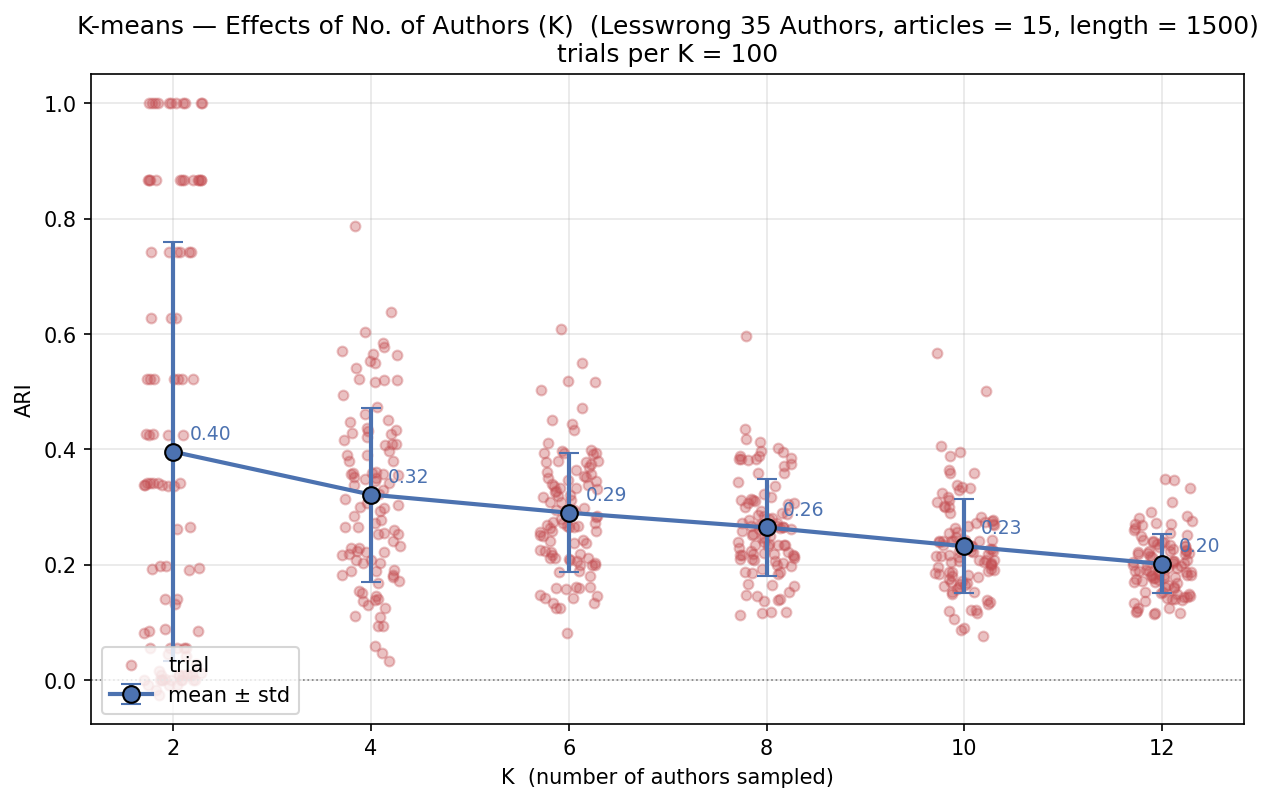
\includegraphics[width=0.82\linewidth]{../src/kmeans/outputs/effect_of_k/ari_vs_k.png}
  \caption{ARI vs.\ $K$ on \texttt{cleaned\_35} ($M=15$, $N=1500$, $100$
  trials per $K$). Mean ARI falls monotonically from $0.40$ at $K=2$ to
  $0.20$ at $K=12$. The spread shrinks rapidly with $K$.}
  \label{fig:k}
\end{figure}

The downward trend is clear and, on this larger author pool, essentially
monotone: mean ARI falls from $0.40$ at $K=2$ to $0.32$ at $K=4$, $0.29$ at
$K=6$, $0.26$ at $K=8$, $0.23$ at $K=10$, and $0.20$ at $K=12$. The slope is
steepest between $K=2$ and $K=4$, then settles into a steady decline of
roughly $0.03$ per additional cluster.

The variance across trials also depends strongly on $K$. At $K=2$ the outcome
is dominated by \emph{which} two authors are drawn: some pairs are near-trivial
to separate and produce ARI close to $1.0$, while others sit at chance. As $K$
grows, each trial draws a more representative slice of the author pool, the
error bars shrink, and the spread is driven more by the intrinsic difficulty
of the task than by author-group luck.

\subsection{\texorpdfstring{Effect of Article Length ($N$)}{Effect of Article Length (N)}}

How does article length $N$ affect performance? Most of our $107$ features are
proportions, frequencies, means: quantities that should be agnostic to length
in expectation, yet noisier when estimated from short articles. We therefore
expect ARI to rise with $N$.

\paragraph{Setup.}
We use \texttt{cleaned\_10} with $K=5$ and $M=15$, sweeping
$N \in \{100, 200, 500, 1000, 1500\}$. For each $N$ we run $50$ trials: sample
$5$ of the $10$ authors, sample $15$ articles per author, truncate to the first
$N$ words, extract features, run K-means.

\begin{figure}[H]
  \centering
  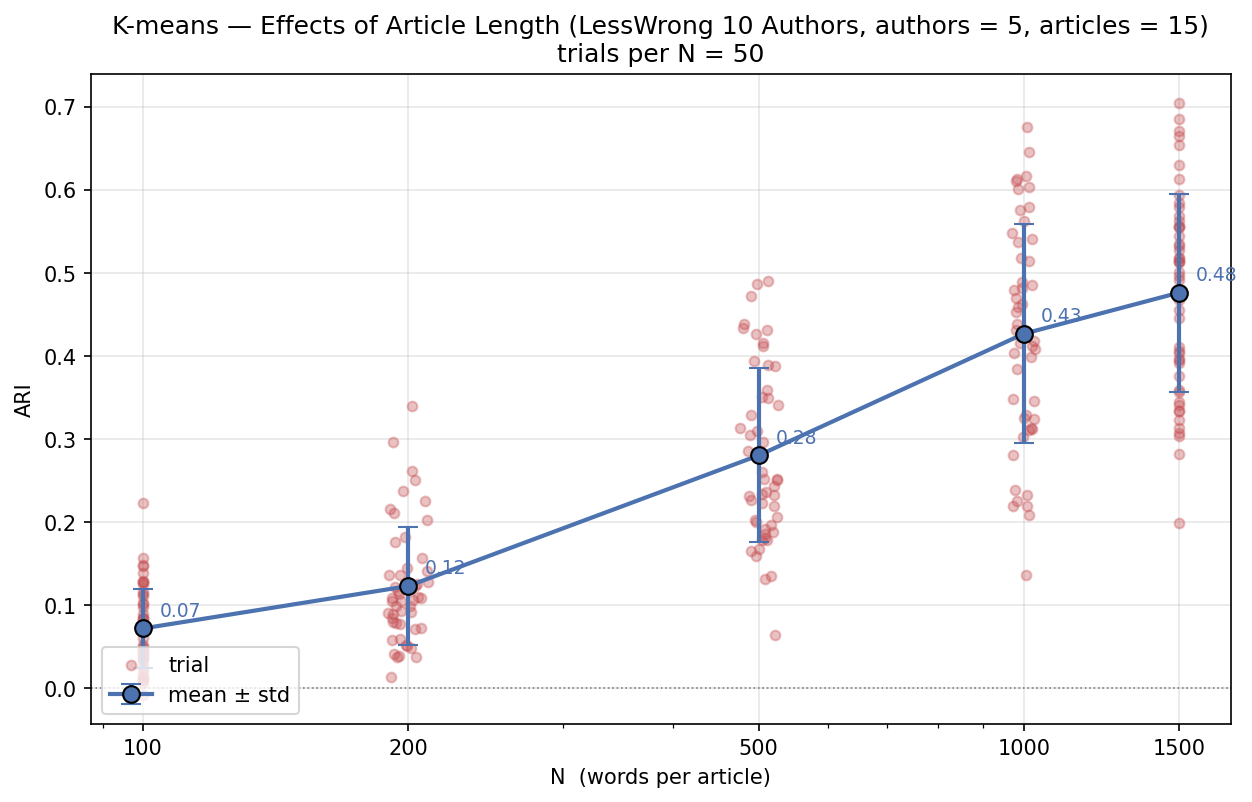
\includegraphics[width=0.82\linewidth]{../src/kmeans/outputs/effect_of_n/ari_vs_n_10authors.png}
  \caption{ARI vs.\ $N$ on \texttt{cleaned\_10} ($K=5$, $M=15$, $50$ trials per
  $N$). ARI rises steeply from $0.07$ at $N=100$ to $0.48$ at $N=1500$.}
  \label{fig:n10}
\end{figure}

The trend is steep: ARI climbs from $0.07$ at $N=100$ to $0.48$ at $N=1500$,
with the slope easing slightly between $N=1000$ and $N=1500$, hinting at a
plateau that has not yet arrived. To see whether the curve really flattens, we
need longer articles. Finding many long ($\geq 3000$-word) articles for ten
LessWrong authors is impractical, so we switch to a separate
\textit{5 Authors} subset for whom we found $35$--$57$ articles each of length
$\geq 3{,}000$ words. The setup is identical except there is no author sampling
(all 5 are used each trial) and $N$ now ranges up to $3{,}000$.

\begin{figure}[H]
  \centering
  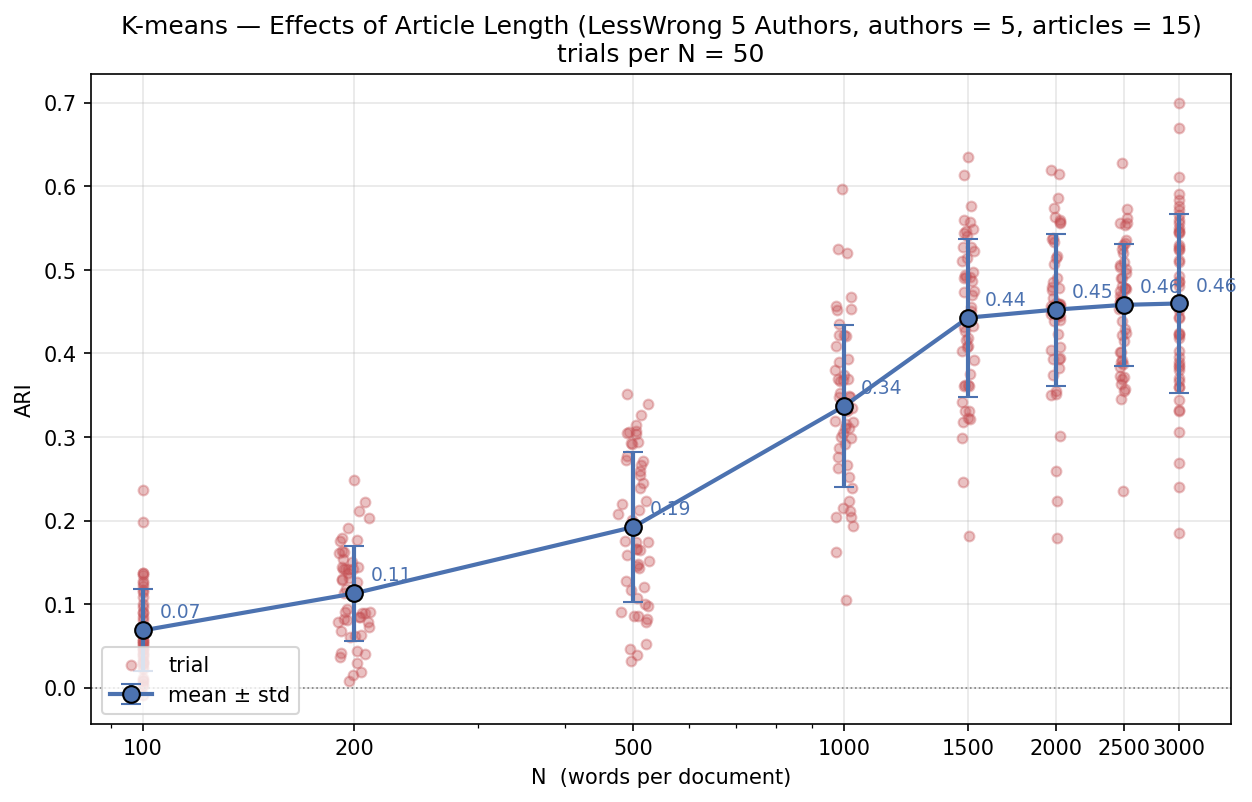
\includegraphics[width=0.82\linewidth]{../src/kmeans/outputs/effect_of_n/ari_vs_n_5authors.png}
  \caption{ARI vs.\ $N$ on the 5-author subset ($K=5$, $M=15$, $50$ trials per
  $N$). The curve follows the 10-author trend up to $N=1500$, then
  \textbf{flattens}: ARI moves only from $0.44$ to $0.46$ over the range
  $N \in \{1500, 2000, 2500, 3000\}$.}
  \label{fig:n5}
\end{figure}

The shape is striking. Up to $N=1500$ the curve mirrors the 10-author result;
past $N=1500$ it hits a clear break point, barely moving from $0.44$ to $0.46$
over the next $1{,}500$ words. A few possible explanations:

\begin{itemize}\setlength\itemsep{2pt}
  \item \textbf{Feature convergence.} By $N=1500$ most rate-based features may
        already be close to their author means, so the algorithm is hitting a
        performance ceiling for this dataset and feature set.
  \item \textbf{Topic shifts within long articles.} Long articles often span
        multiple sub-discussions; transitions between them can shift the
        stylistic surface. Since we truncate articles from the beginning to
        the first $N$ words, the break point may reflect an implicit average
        coherent-stretch length of roughly $1{,}500$ words.
  \item \textbf{Noisy tails.} Authors often write discursively at the start
        and then move into code blocks, image captions, math, and quoted
        material, all of which add noise to the features.
  \item \textbf{Dataset-specific.} The break point may simply be a property
        of this particular five-author group rather than a general pattern.
\end{itemize}

Regardless, the practical implication is the same: there is little to gain
from chasing articles longer than $\sim 1{,}500$ words for this kind of
clustering problem.

\paragraph{Why does the curve rise in the first place?}
Of our $107$ features, roughly $100$ are proportions, rates, means, or
medians. For each author, these features can be viewed as draws from an
underlying author-specific stylistic distribution that is largely independent
of article length. By the Law of Large Numbers, the observed feature values
converge toward the author's true means as sample size increases. At small $N$
each feature is a noisy estimate of the underlying rate, causing articles from
different authors to overlap in feature space.

To make this concrete, we isolate author \code{zvi} from the 5-author subset
and track two features as a function of article length:

\begin{enumerate}\setlength\itemsep{1pt}
  \item Concatenate all of \code{zvi}'s articles into a single ``master''
        document.
  \item For each window size $N \in \{100, 200, 500, 1000, 1500, 2000, 2500,
        3000\}$, draw $20$ random contiguous slices of exactly $N$ words.
  \item Compute \code{fw\_you} (rate of the word ``you'') and
        \code{word\_len\_1\_frac} (rate of one-character words) on each
        slice.
\end{enumerate}

\begin{figure}[H]
  \centering
  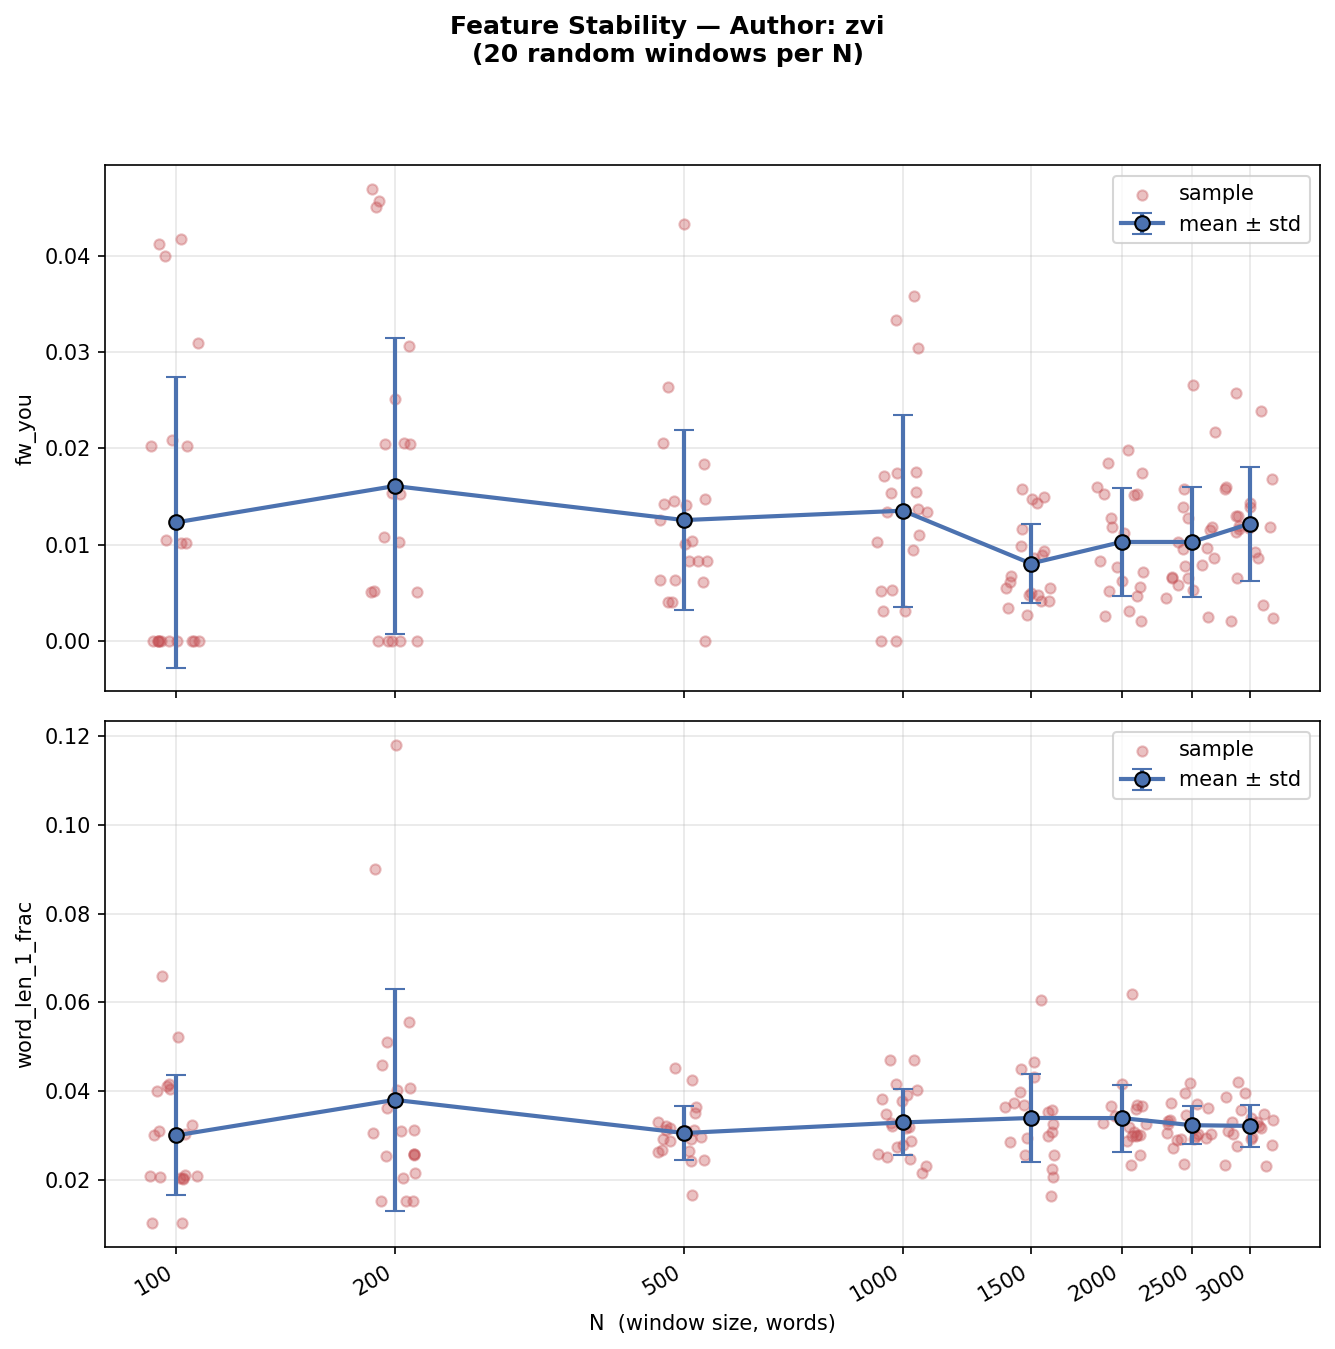
\includegraphics[width=0.75\linewidth]{../src/kmeans/outputs/effect_of_n/feature_stability_zvi.png}
  \caption{Two stylometric features computed on random windows of \code{zvi}'s
  concatenated text. The spread around each mean narrows as $N$ grows.}
  \label{fig:feat_stability}
\end{figure}

The standard deviation of both features is large at small $N$ and generally
shrinks as $N$ increases. At $N=100$ each window is too short to yield a
reliable estimate of \code{zvi}'s rates; by $N=1500$ the estimates have
stabilised.

\subsection{Effect of Era}

Our decision to collect equal numbers of articles from $\leq 2022$ and
$\geq 2024$ in the \texttt{cleaned\_10} dataset stems from a practical
observation. ChatGPT and similar chatbots emerged in late $2022$ and quickly
gained traction as writing assistants. By $2024$ they were routine tools for
many writers, used to proofread or polish blog posts, emails, and similar
texts. Chatbots have a distinctive style of their own; if a substantial
fraction of authors run their drafts through one, individual writing styles
might homogenise. We therefore hypothesised \textbf{lower K-means performance
in the post-2024 era than in the pre-2022 era}.

\paragraph{Setup.}
\texttt{cleaned\_10}, $K=4$, $M=10$, $N=1{,}500$, $50$ trials per era. Each
trial samples $4$ of the $10$ authors and $10$ of each author's $20$
era-restricted articles; the rest of the pipeline is unchanged.

\begin{figure}[H]
  \centering
  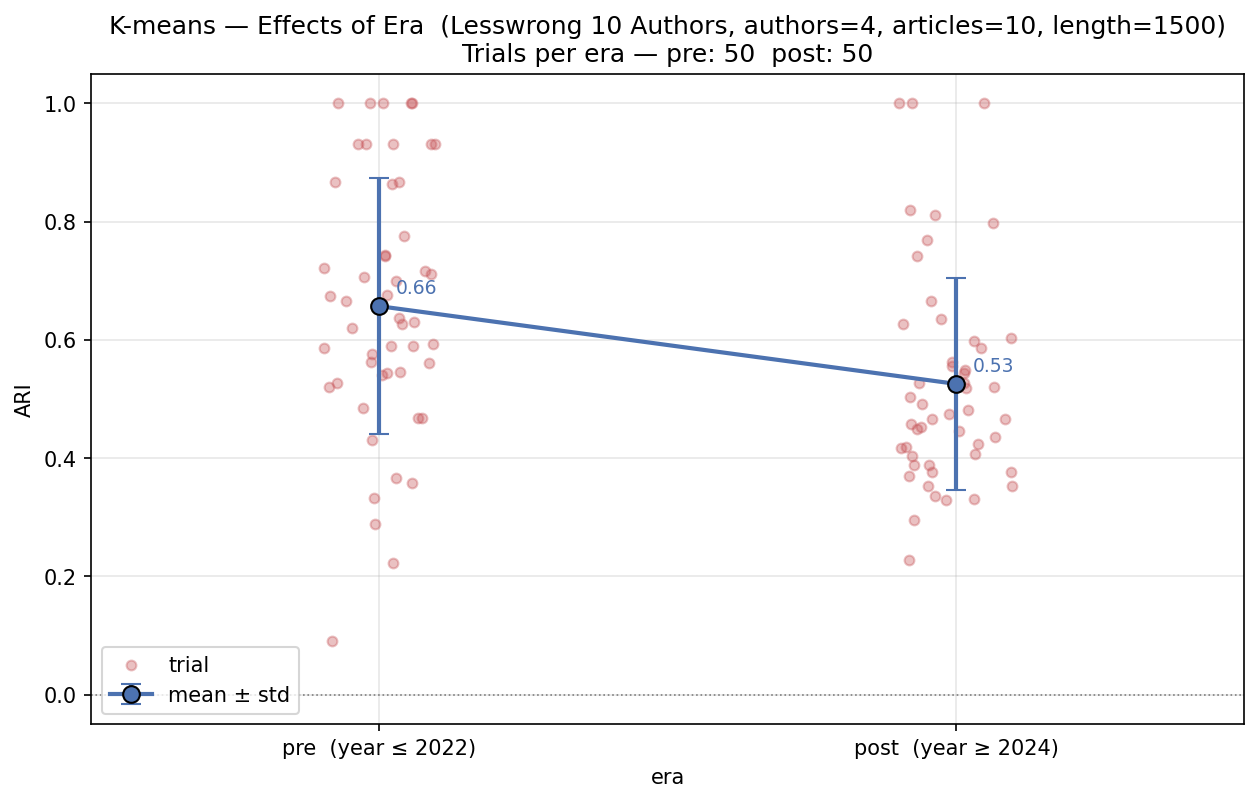
\includegraphics[width=0.82\linewidth]{../src/kmeans/outputs/effect_of_era/ari_vs_era.png}
  \caption{ARI by era ($K=4$, $M=10$, $N=1500$, $50$ trials per era). Mean ARI
  drops from \textbf{$0.66$} in the pre-$2022$ era to \textbf{$0.53$} in the
  post-$2024$ era.}
  \label{fig:era}
\end{figure}

The mean ARI drops from \textbf{$0.66$} (pre, $\leq 2022$) to \textbf{$0.53$}
(post, $\geq 2024$), a substantial gap that is consistent with our
expectation.

\paragraph{Does this prove people are using AI to polish their writing?}
Unfortunately, no. The drop is too large to dismiss as noise, but AI use is
only one of several plausible explanations:

\begin{itemize}\setlength\itemsep{2pt}
  \item \textbf{Writing evolves.} Style is not static. An author's prose today
        may not mirror their prose from five years ago simply because they
        have grown intellectually and socially.
  \item \textbf{Topic shifts on LessWrong.} The community's focus has changed
        in response to current events. For instance, \code{kaj\_sotala}'s
        pre-$2023$ articles are mostly about biology, social dynamics, and
        self-improvement, while his post-$2023$ articles are mostly about AI.
        A shift in topic mix can drag stylistic features along with it.
\end{itemize}

The era effect is real and worth noting; however, attributing it specifically
to AI-assisted writing would require a controlled study that this experiment
cannot deliver.

% =============================================================================
\section{Authorship Verification with SVM}
\label{sec:svm}

\textit{K-means asked whether style \emph{clusters}. We now ask a
supervised question: given two articles, were they written by the same person?
This is authorship verification, and unlike multi-class identification it does
not require the model to have ever seen the candidate authors before. A good
verifier learns ``what same-author style looks like'' in the abstract, then
applies that to new pairs.}

\subsection{Reframing as Same-Author Detection}

The verification framing changes what the model has to learn. A classifier
that names an author has to memorise each author's fingerprint individually
--- it cannot generalise to people not in its training set. A verifier instead
learns a single decision rule: \textit{do these two fingerprints match?} If
that rule is genuinely about style rather than topic, the same model should
work on author pairs it has never seen. To test that, we will deliberately
arrange the data so that the authors at evaluation time are disjoint from
the authors used to train and tune.

\subsection{Support Vector Machines and the RBF Kernel}

A Support Vector Machine (SVM) is a supervised classifier that places a
decision boundary --- a \emph{hyperplane} --- through feature space, choosing
the hyperplane that leaves the widest possible margin on either side. When the
data are not linearly separable, the SVM uses a \textbf{kernel} to implicitly
map the inputs into a higher-dimensional space where a hyperplane may exist.
We use the \textbf{Radial Basis Function (RBF)} kernel
\[
  K(x_{i},x_{j}) = \exp\!\bigl(-\gamma \lVert x_{i}-x_{j} \rVert^{2}\bigr),
\]
which can be read as a similarity score: $K$ is near $1$ when two vectors are
close in Euclidean distance and near $0$ when they are far apart. Two
hyperparameters control the model:

\begin{itemize}\setlength\itemsep{2pt}
  \item \textbf{$C$} --- the regularisation strength. A small $C$ tolerates
        misclassified training points in exchange for a wider, smoother
        margin; a large $C$ insists on classifying every training point
        correctly, often at the cost of overfitting.
  \item \textbf{$\gamma$} --- the kernel width. A large $\gamma$ makes the
        Gaussian sharp, so each support vector only influences its immediate
        neighbourhood, producing wiggly, locally fitted decision regions and
        again risking overfitting. A small $\gamma$ stretches each support
        vector's influence over a wide region, giving a smooth, almost linear
        boundary that may underfit.
\end{itemize}

Figure~\ref{fig:svm_concept} sketches these intuitions visually.

\begin{figure}[H]
\centering
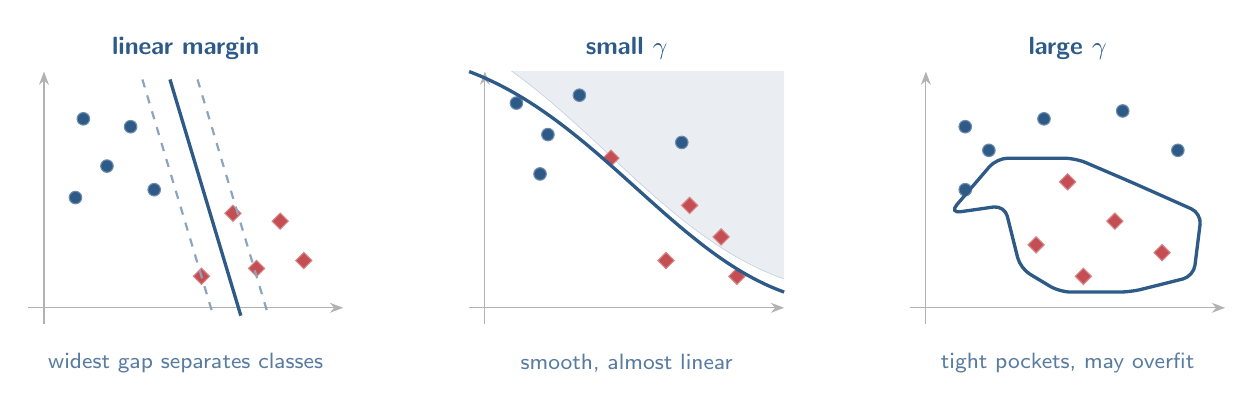
\begin{tikzpicture}[
  cls0/.style={circle, fill=accent, draw=accent!70, inner sep=1.6pt},
  cls1/.style={diamond, fill=accentred, draw=accentred!70, inner sep=1.5pt},
  ax/.style={->, >=Stealth, gray!60, thin},
  hp/.style={accent, very thick},
  marg/.style={accent!55, dashed, thick},
  region/.style={accent!10, draw=accent!30, very thin, rounded corners=2pt},
  caption/.style={font=\footnotesize\sffamily, text=accent!80},
]

% Panel 1: linear margin
\begin{scope}
  \node[font=\small\sffamily\bfseries, text=accent] at (1.8, 3.3)
    {linear margin};
  \draw[ax] (-0.2,0) -- (3.8,0);
  \draw[ax] (0,-0.2) -- (0,3.0);
  % class 0 (blue)
  \node[cls0] at (0.5,2.4) {};
  \node[cls0] at (0.8,1.8) {};
  \node[cls0] at (1.1,2.3) {};
  \node[cls0] at (1.4,1.5) {};
  \node[cls0] at (0.4,1.4) {};
  % class 1 (red)
  \node[cls1] at (2.4,1.2) {};
  \node[cls1] at (2.7,0.5) {};
  \node[cls1] at (3.0,1.1) {};
  \node[cls1] at (3.3,0.6) {};
  \node[cls1] at (2.0,0.4) {};
  % hyperplane + margin
  \draw[hp] (1.6,2.9) -- (2.5,-0.1);
  \draw[marg] (1.25,2.9) -- (2.15,-0.1);
  \draw[marg] (1.95,2.9) -- (2.85,-0.1);
  \node[caption] at (1.8, -0.7) {widest gap separates classes};
\end{scope}

% Panel 2: small gamma (smooth boundary)
\begin{scope}[xshift=5.6cm]
  \node[font=\small\sffamily\bfseries, text=accent] at (1.8, 3.3)
    {small $\gamma$};
  \draw[ax] (-0.2,0) -- (3.8,0);
  \draw[ax] (0,-0.2) -- (0,3.0);
  \begin{scope}
    \clip (-0.2,-0.2) rectangle (3.8,3.0);
    \fill[region]
      (-0.5,3.5) .. controls (1.4,2.6) and (2.4,0.5) .. (4.5,0.2)
      -- (4.5,3.5) -- cycle;
  \end{scope}
  % class 0 (blue) - upper-left region
  \node[cls0] at (0.4,2.6) {};
  \node[cls0] at (0.8,2.2) {};
  \node[cls0] at (1.2,2.7) {};
  \node[cls0] at (0.7,1.7) {};
  % class 1 (red) - lower-right region
  \node[cls1] at (2.6,1.3) {};
  \node[cls1] at (3.0,0.9) {};
  \node[cls1] at (2.3,0.6) {};
  \node[cls1] at (3.2,0.4) {};
  % outliers near boundary
  \node[cls1] at (1.6,1.9) {};
  \node[cls0] at (2.5,2.1) {};
  \draw[hp]
    (-0.2,3.0) .. controls (1.4,2.4) and (2.4,0.7) .. (3.8,0.2);
  \node[caption] at (1.8, -0.7) {smooth, almost linear};
\end{scope}

% Panel 3: large gamma (wiggly boundary)
\begin{scope}[xshift=11.2cm]
  \node[font=\small\sffamily\bfseries, text=accent] at (1.8, 3.3)
    {large $\gamma$};
  \draw[ax] (-0.2,0) -- (3.8,0);
  \draw[ax] (0,-0.2) -- (0,3.0);
  % class 0 (blue) clusters
  \node[cls0] at (0.5,2.3) {};
  \node[cls0] at (0.8,2.0) {};
  \node[cls0] at (0.5,1.5) {};
  \node[cls0] at (1.5,2.4) {};
  \node[cls0] at (2.5,2.5) {};
  \node[cls0] at (3.2,2.0) {};
  % class 1 (red)
  \node[cls1] at (1.8,1.6) {};
  \node[cls1] at (1.4,0.8) {};
  \node[cls1] at (2.4,1.1) {};
  \node[cls1] at (3.0,0.7) {};
  \node[cls1] at (2.0,0.4) {};
  % wiggly tight contour around red points
  \draw[hp, rounded corners=4pt]
    (0.3,1.2) -- (1.0,1.3) -- (1.2,0.5) -- (1.7,0.2)
    -- (2.6,0.2) -- (3.4,0.4) -- (3.5,1.2) -- (2.6,1.6)
    -- (1.9,1.9) -- (0.9,1.9) -- cycle;
  \node[caption] at (1.8, -0.7) {tight pockets, may overfit};
\end{scope}

\end{tikzpicture}
\caption{Intuition for the SVM with an RBF kernel. \textit{Left}: in
linearly separable feature space the SVM picks the hyperplane with the widest
margin (dashed). \textit{Middle and right}: changing $\gamma$ trades off
generality for locality. A small $\gamma$ gives a smooth boundary that may
underfit; a large $\gamma$ wraps tightly around training points and tends to
overfit.}
\label{fig:svm_concept}
\end{figure}

\subsection{Data Preparation}

\paragraph{Dataset.}
We work with the \texttt{cleaned\_35} corpus from Section~\ref{sec:data}:
$1{,}484$ articles across $35$ distinct authors (per-author counts in
Table~\ref{tab:dataset_c35}).

\paragraph{Author-based split.}
If we shuffled article pairs into training and test sets at random, articles
written by the same author would routinely appear in both sets. The model
would then learn each author's specific fingerprint rather than a generic
``same-author vs.\ different-author'' rule, and the test accuracy would
overstate how well it generalises to new authors --- a classic case of data
leakage. We avoid this by splitting at the \emph{author} level: $80\%$ of the
authors ($28$) go to the training pool and the remaining $20\%$ ($7$) form a
test pool of authors the model has never seen. Every pair is generated from
within a single pool, so the train and test pairs are guaranteed to involve
disjoint people.

\paragraph{Pair construction.}
Verification needs to take \emph{two} articles as input. Given articles $1$
and $2$ with $107$-dimensional feature vectors $f_{1}$ and $f_{2}$, we form a
single $321$-dimensional pair feature by concatenating three element-wise
combinations:
\begin{itemize}\setlength\itemsep{1pt}
  \item $|f_{1} - f_{2}|$ --- absolute difference: where do the two authors
        diverge most strongly?
  \item $(f_{1} - f_{2})^{2}$ --- squared difference: emphasise the largest
        divergences over the small ones.
  \item $f_{1} \odot f_{2}$ --- element-wise product: high only when
        \emph{both} articles strongly exhibit the same trait, which the two
        difference operators cannot distinguish from ``neither uses the
        trait''.
\end{itemize}
Figure~\ref{fig:svm_pipeline} shows how this assembles into the SVM input.

\begin{figure}[H]
\centering
\resizebox{\linewidth}{!}{%
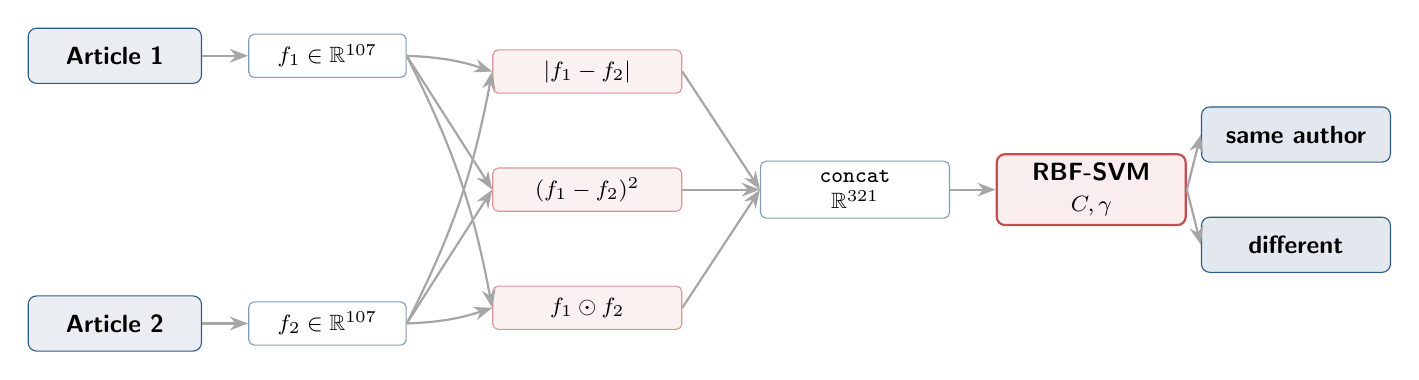
\begin{tikzpicture}[
  art/.style={draw=accent, fill=accent!10, rounded corners=3pt,
    minimum width=2.2cm, minimum height=0.7cm,
    align=center, font=\small\sffamily\bfseries},
  feat/.style={draw=accent!60, fill=white, rounded corners=2pt,
    minimum width=2.0cm, minimum height=0.55cm,
    align=center, font=\footnotesize\ttfamily},
  op/.style={draw=accentred!60, fill=accentred!8, rounded corners=2pt,
    minimum width=2.4cm, minimum height=0.55cm,
    align=center, font=\footnotesize\sffamily},
  svmbox/.style={draw=accentred, fill=accentred!10, rounded corners=3pt,
    minimum width=2.4cm, minimum height=0.9cm,
    align=center, font=\small\sffamily\bfseries, thick},
  outbox/.style={draw=accent, fill=accent!14, rounded corners=3pt,
    minimum width=2.4cm, minimum height=0.7cm,
    align=center, font=\small\sffamily\bfseries},
  arr/.style={->, >=Stealth, gray!70, thick},
]
% articles
\node[art] (a1) at (0, 1.7) {Article 1};
\node[art] (a2) at (0, -1.7) {Article 2};
% feature vectors
\node[feat] (f1) at (2.7, 1.7) {$f_{1} \in \mathbb{R}^{107}$};
\node[feat] (f2) at (2.7, -1.7) {$f_{2} \in \mathbb{R}^{107}$};
\draw[arr] (a1) -- (f1);
\draw[arr] (a2) -- (f2);
% three operations
\node[op] (op1) at (6.0, 1.5)  {$|f_{1}-f_{2}|$};
\node[op] (op2) at (6.0, 0.0)  {$(f_{1}-f_{2})^{2}$};
\node[op] (op3) at (6.0, -1.5) {$f_{1}\odot f_{2}$};
\draw[arr] (f1.east) to[bend left=8]  (op1.west);
\draw[arr] (f2.east) to[bend right=8] (op1.west);
\draw[arr] (f1.east) -- (op2.west);
\draw[arr] (f2.east) -- (op2.west);
\draw[arr] (f1.east) to[bend left=8]  (op3.west);
\draw[arr] (f2.east) to[bend right=8] (op3.west);
% concat
\node[feat, minimum width=2.4cm] (cat) at (9.4, 0)
  {concat\\ $\mathbb{R}^{321}$};
\draw[arr] (op1.east) -- (cat.west);
\draw[arr] (op2.east) -- (cat.west);
\draw[arr] (op3.east) -- (cat.west);
% SVM
\node[svmbox] (svm) at (12.4, 0) {RBF-SVM\\ \footnotesize $C,\gamma$};
\draw[arr] (cat) -- (svm);
% output
\node[outbox] (yhat) at (15.0, 0.7) {same author};
\node[outbox] (yhatn) at (15.0, -0.7) {different};
\draw[arr] (svm.east) -- (yhat.west);
\draw[arr] (svm.east) -- (yhatn.west);
\end{tikzpicture}%
}
\caption{The SVM verification pipeline. Two articles are reduced to their
$107$ stylometric features, combined three ways into a $321$-dimensional pair
vector, scaled, and fed to an RBF-SVM that outputs a same/different
prediction.}
\label{fig:svm_pipeline}
\end{figure}

\paragraph{Class balance.}
The resulting pairwise dataset is strictly balanced, exactly $50\%$ positive
(same-author, label $1$) and $50\%$ negative (different-author, label $0$).
Positive pairs are formed by taking combinations of articles within a single
author; to keep authors with many articles from dominating, we cap positives
at $200$ pairs per author and sample uniformly when that cap is exceeded.
Negative pairs are formed by sampling two distinct authors uniformly at
random and one article from each, matching the total positive count.

\subsection{Hyperparameter Tuning}

\paragraph{Why a custom grid search.}
The off-the-shelf \code{GridSearchCV} would split rows at the pair level, which
re-introduces the same leakage we eliminated at the train/test boundary --- a
fold's validation pair could share an author with a training pair. We
therefore run the cross-validation \emph{at the author level}:

\begin{itemize}\setlength\itemsep{2pt}
  \item \textbf{5-fold author-CV.} The training authors are partitioned into
        five disjoint folds. Each round uses four folds for training and one
        for validation; no author appears in both halves of any round.
  \item \textbf{Fold-wise pair generation and scaling.} Pair construction
        happens \emph{inside} each fold, after the author split. The
        \code{StandardScaler} ($z = (x-\mu)/\sigma$) is fit on the training
        pairs of the fold and applied to the validation pairs.
  \item \textbf{Grid.} We sweep $C \in \{0.1, 1, 10\}$ and
        $\gamma \in \{0.001, 0.01, 0.1\}$, and repeat the whole pipeline over
        five random seeds ($19$ through $23$) so the reported numbers are
        stable.
\end{itemize}

\paragraph{Results.}
Table~\ref{tab:gridsearch} reports mean training accuracy, mean validation
accuracy, and the generalisation gap (train minus val) for every cell of the
grid.

\begin{table}[H]
  \centering
  \small
  \caption{SVM hyperparameter grid, aggregated across $5$ seeds.}
  \label{tab:gridsearch}
  \begin{tabular}{@{}llcccl@{}}
    \toprule
    \textbf{$C$} & \textbf{$\gamma$} & \textbf{Train acc} & \textbf{Val acc}
        & \textbf{Gap} & \textbf{Observation} \\
    \midrule
    $0.1$ & $0.001$ & $0.7657\pm0.0047$ & $0.7284\pm0.0050$ & $0.0373$
        & Most stable (lowest gap) \\
    $0.1$ & $0.01$  & $0.6909\pm0.0019$ & $0.6105\pm0.0081$ & $0.0804$
        & Underfitting \\
    $0.1$ & $0.1$   & $1.0000\pm0.0000$ & $0.5000\pm0.0000$ & $0.5000$
        & Overfitting \\
    $1$   & $0.001$ & $0.8398\pm0.0042$ & $0.7327\pm0.0072$ & $0.1070$
        & Highest val accuracy \\
    $1$   & $0.01$  & $0.9954\pm0.0005$ & $0.6942\pm0.0073$ & $0.3012$
        & Overfitting \\
    $1$   & $0.1$   & $1.0000\pm0.0000$ & $0.5001\pm0.0003$ & $0.4999$
        & Overfitting \\
    $10$  & $0.001$ & $0.9585\pm0.0023$ & $0.7204\pm0.0052$ & $0.2380$
        & Overfitting \\
    $10$  & $0.01$  & $1.0000\pm0.0000$ & $0.6907\pm0.0061$ & $0.3093$
        & Overfitting \\
    $10$  & $0.1$   & $1.0000\pm0.0000$ & $0.5002\pm0.0004$ & $0.4998$
        & Overfitting \\
    \bottomrule
  \end{tabular}
\end{table}

The pattern matches the geometric intuition from
Figure~\ref{fig:svm_concept}. Large $\gamma$ produces $100\%$ training accuracy
and chance-level validation accuracy --- the kernel's Gaussian bumps are tight
enough to memorise each training pair without generalising. Large $C$ with
moderate $\gamma$ does the same thing for a slightly different reason: the
penalty for misclassifying any training pair is so high that the optimiser
sacrifices margin width to fit them all. After ruling out these degenerate
configurations two candidates remain:

\begin{itemize}\setlength\itemsep{1pt}
  \item \textbf{Configuration A} ($C=1$, $\gamma=0.001$): val acc
        $73.27\%$, gap $10.7\%$.
  \item \textbf{Configuration B} ($C=0.1$, $\gamma=0.001$): val acc
        $72.84\%$, gap $3.73\%$.
\end{itemize}

\noindent We pick \textbf{Configuration B}. Although Configuration A wins on
raw validation accuracy by a fraction of a percent, its generalisation gap is
nearly three times larger. The smaller gap of Configuration B suggests it is
extracting a more robust signal, which we expect to matter when we evaluate on
a fresh set of authors.

\subsection{Final Evaluation}

After hyperparameter tuning, we retrain the final SVM using the chosen
configuration ($C{=}0.1$, $\gamma{=}0.001$) on the \emph{complete} training
set --- the $11{,}200$ pairs generated from all $28$ training authors,
scaled with a fresh \code{StandardScaler} fit on those pairs. The retrained
model is then evaluated once on the test set: the $2{,}800$ pairs generated
from the held-out $7$ test authors, never seen during training or tuning.
The whole procedure (retrain + test) is repeated across the same five seeds
($19$ through $23$) used in the tuning stage.

\begin{table}[H]
  \centering
  \small
  \caption{Test-set metrics for the selected SVM ($C=0.1$, $\gamma=0.001$)
  across $5$ seeds. Macro precision/recall/F1 are unweighted means over the
  two classes.}
  \label{tab:finaleval}
  \begin{tabular}{@{}lccccc@{}}
    \toprule
    \textbf{Seed} & \textbf{Accuracy} & \textbf{Macro P}
        & \textbf{Macro R} & \textbf{Macro F1} & \textbf{ROC-AUC} \\
    \midrule
    19 & $0.7439$ & $0.74$ & $0.74$ & $0.74$ & $0.8234$ \\
    20 & $0.7350$ & $0.74$ & $0.73$ & $0.73$ & $0.8164$ \\
    21 & $0.6989$ & $0.70$ & $0.70$ & $0.70$ & $0.7823$ \\
    22 & $0.7393$ & $0.75$ & $0.74$ & $0.74$ & $0.8386$ \\
    23 & $0.7461$ & $0.75$ & $0.75$ & $0.74$ & $0.8086$ \\
    \midrule
    \textbf{Mean $\pm$ Std} & \textbf{$0.7326\pm0.0189$}
        & \textbf{$0.7360\pm0.0207$} & \textbf{$0.7320\pm0.0205$}
        & \textbf{$0.7300\pm0.0187$} & \textbf{$0.8139\pm0.0186$} \\
    \bottomrule
  \end{tabular}
\end{table}

The most striking property of these numbers is how tight they are. Five
completely different splits of test authors produce accuracies within a
two-percentage-point band, and a single-decimal-place range of ROC-AUC.
That stability is the payoff for splitting at the author level: we are
measuring a property of the model rather than of any one author group. The
weakest run (seed 21, ROC-AUC $0.7823$) presumably drew a test pool with
authors who are stylistically similar to one another or unusually similar to
some training-pool authors, but even that pessimistic case lies well above
chance.

The agreement among accuracy ($0.7326$), macro precision ($0.7360$), macro
recall ($0.7320$), and macro F1 ($0.7300$) is the second indicator worth
noting --- the classifier is not preferring one class over the other; it is
balanced on both kinds of mistake.

\paragraph{ROC curves.}
\begin{figure}[H]
  \centering
  \includegraphics[width=0.78\linewidth]%
    {\detokenize{../src/svm&logisticregression/outputs/ROC_svm.png}}
  \caption{Receiver Operating Characteristic curves of the selected SVM across
  the five seeds.}
  \label{fig:roc_svm}
\end{figure}

The ROC curves trace the trade-off between true-positive rate and
false-positive rate as the decision threshold is varied. All five curves sit
well above the diagonal, with seed 22 reaching ROC-AUC $0.8386$ (the easiest
test pool) and seed 21 trailing at $0.7823$ (the hardest). The mean of
$0.8139$ summarises the SVM's discriminative ability across operating points,
not just at the default threshold.

\paragraph{Confusion matrix.}
\begin{table}[H]
  \centering
  \small
  \caption{Confusion matrix averaged across the five seeds.}
  \label{tab:confmatrix}
  \begin{tabular}{lcc}
    \toprule
    \textbf{Actual \textbackslash\ Predicted} & \textbf{Different ($0$)} & \textbf{Same ($1$)} \\
    \midrule
    \textbf{Different ($0$)} & $1002.8$ (TN) & $397.2$ (FP) \\
    \textbf{Same ($1$)}      & $351.4$ (FN)  & $1048.6$ (TP) \\
    \bottomrule
  \end{tabular}
\end{table}

Errors are roughly symmetric: $397$ false positives versus $351$ false
negatives per run on average. Two qualitative stories emerge from sampling
those errors. False positives tend to involve two different authors who
inhabit overlapping stylistic conventions --- formal academic register, shared
jargon, common essay structure --- which inflates the element-wise product
$f_{1}\odot f_{2}$ even when the underlying voices are distinct. False
negatives are the mirror case: a single author writing across registers,
audiences, or moods. The same author writing a technical analysis and a
personal essay produces $|f_{1}-f_{2}|$ values that look more like two
different people than like one.

\subsection{Comparison with a Logistic Regression Baseline}

A natural question is how much of the SVM's performance comes from the kernel
rather than from the engineered pair features. To check, we run the entire
pipeline a second time with the SVM swapped out for a logistic regression
(L2 regularised, default $C=1$). Same authors splits, same pair construction,
same scaler, same seeds.

\begin{table}[H]
\centering
\small
\caption{Logistic regression vs.\ RBF-SVM on the same test pipeline.}
\label{tab:comparison_lr_svm}
\begin{tabular}{lcc}
\toprule
\textbf{Metric} & \textbf{Logistic regression} & \textbf{RBF-SVM} \\
\midrule
Accuracy        & $72.21 \pm 2.11$ & $73.26 \pm 1.89$ \\
Macro precision & $72.80 \pm 2.39$ & $73.60 \pm 2.07$ \\
Macro recall    & $72.20 \pm 2.05$ & $73.20 \pm 2.05$ \\
Macro F1        & $72.00 \pm 2.12$ & $73.00 \pm 1.87$ \\
ROC-AUC         & $79.38 \pm 2.89$ & $81.39 \pm 1.86$ \\
\bottomrule
\end{tabular}
\end{table}

The RBF-SVM wins on every metric, but only narrowly: roughly $1$ percentage
point of accuracy and macro F1, and $2$ points of ROC-AUC. Logistic
regression --- a strictly linear model in the pair-feature space --- is
already pulling out most of the available signal. This tells us two things.
First, the engineered pair features are doing the heavy lifting: by the time
$|f_{1}-f_{2}|$, $(f_{1}-f_{2})^{2}$, and $f_{1}\odot f_{2}$ have been
stacked together, the same/different boundary is mostly linear. Second, the
RBF kernel is genuinely capturing some non-linear structure --- the
improvement is small but consistent across all five seeds --- so the
non-linearity exists, just not in a way that dominates.

The practical implication is the standard one: pick whichever side of the
complexity/performance trade-off matters more for the application. The SVM is
the better predictor; the logistic regression is faster, smaller, and easier
to inspect.

% =============================================================================
\section{Author Identification with a Neural Network}
\label{sec:nn}

\textit{The verification model gave us a pairwise yes/no. We now ask: given a article, can a model name its
author from a closed list of candidates, or correctly refuse if the article is
from someone outside the list?}

\subsection{The Task}

A five-author classifier would assume that every article was written by one
of those five. In the real world that assumption fails: a article may come
from someone the model has never seen, and a five-author model will
confidently mislabel it as whichever known author it resembles most. We
therefore treat this as a plain \textbf{six-class} classification problem:
the five known LessWrong authors plus an explicit sixth class,
\code{none\_of\_the\_5\_authors}, that the network must learn to recognise.

\subsection{Dataset and Preprocessing}

The five known authors --- drawn from \texttt{cleaned\_5}
(Table~\ref{tab:dataset_cleaned_5}) --- are \code{Eliezer Yudkowsky},
\code{John Wentworth}, \code{Raemon}, \code{Scott Alexander}, and \code{Zvi},
contributing roughly $150$ articles each for $723$ in total. The ``none''
class is built from $15$ other LessWrong authors (\code{ricraz},
\code{benquo}, \code{abramdemski}, \code{sarahconstantin},
\code{holdenkarnofsky}, \code{gordon-seidoh-worley}, \code{screwtape},
\code{buck}, \code{turntrout}, \code{nunosempere}, \code{benito},
\code{petermccluskey}, \code{joe-carlsmith}, \code{adamshimi}, \code{tsvibt}),
sampling $10$ articles from each for $150$ ``none'' articles. Merged, this
gives \textbf{$873$ articles over $6$ classes}.

From each article we extract the same $107$ stylometric features described in
Section~\ref{sec:kmeans}. Every feature is z-scored with \code{sklearn}'s
\code{StandardScaler}. Crucially, the scaler is fit on the training split only
and then applied to validation and test, so no test-set statistics leak into
training.

\subsection{The Classifier}

A neural network maps a feature vector $\mathbf{x}\in\mathbb{R}^{107}$ to a
probability over $K=6$ classes. Each hidden layer applies an affine transform
followed by the \textbf{ReLU} non-linearity,
\[
  \mathbf{h}^{(\ell)} = \mathrm{ReLU}\!\big(W^{(\ell)}\mathbf{h}^{(\ell-1)}
  + \mathbf{b}^{(\ell)}\big),
  \qquad \mathrm{ReLU}(z)=\max(0,z),
\]
with $\mathbf{h}^{(0)}=\mathbf{x}$. The final layer produces $K$ logits that a
\textbf{softmax} turns into class probabilities,
\[
  p_k(\mathbf{x}) = \frac{\exp(z_k)}{\sum_{j=1}^{K}\exp(z_j)},
\]
and training minimises the multi-class \textbf{cross-entropy} loss over the
training articles,
\[
  L = -\frac{1}{N}\sum_{i=1}^{N}\sum_{k=1}^{K}
      \mathbf{1}[y_i = k]\,\log p_k(\mathbf{x}_i).
\]
Weights are learned by backpropagation with the \textbf{Adam} optimiser
(\code{MLPClassifier} with \code{solver="adam"}). All hidden layers use $64$
units; we vary only the \emph{number} of such layers.

\begin{figure}[H]
\centering
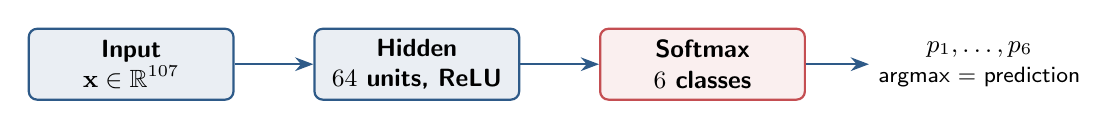
\begin{tikzpicture}[
  node distance=10mm,
  layer/.style={draw=accent, fill=accent!10, rounded corners=3pt,
    minimum width=2.6cm, minimum height=0.9cm, align=center,
    font=\small\sffamily\bfseries, thick},
  outlayer/.style={draw=accentred, fill=accentred!9, rounded corners=3pt,
    minimum width=2.6cm, minimum height=0.9cm, align=center,
    font=\small\sffamily\bfseries, thick},
  arr/.style={->, >=Stealth, accent, thick},
]
  \node[layer]    (in)  {Input\\$\mathbf{x}\in\mathbb{R}^{107}$};
  \node[layer, right=of in]  (h) {Hidden\\$64$ units, ReLU};
  \node[outlayer, right=of h] (out) {Softmax\\$6$ classes};
  \node[draw=none, right=8mm of out, font=\small\sffamily, align=center]
    (p) {$p_1,\dots,p_6$\\\footnotesize argmax = prediction};
  \draw[arr] (in)  -- (h);
  \draw[arr] (h)   -- (out);
  \draw[arr] (out) -- (p);
\end{tikzpicture}
\caption{The winning architecture: a single hidden layer of $64$ ReLU units
feeding a $6$-way softmax (five known authors plus ``none''). Deeper variants
stack more $64$-unit layers between input and output
(Section~\ref{ssec:depth}).}
\label{fig:arch}
\end{figure}

\subsection{Training Protocol}

We split the $873$ articles \textbf{$60/20/20$} (train / validation / test),
stratified by class, and use the validation split to choose a model before
ever touching the test split. Specifically we grid-search over three feature
subsets (the top $30$, top $50$, and all $107$ features) crossed with four
network depths, training each combination on the train split and scoring it
on validation. The winner is then \textbf{retrained on train$+$validation
combined} and evaluated \emph{once} on the held-out test set.

\paragraph{Which features?}
The top-$30$ and top-$50$ subsets are the most informative features as ranked
by \textbf{Random Forest permutation importance}: we fit a random forest
(\code{n\_estimators=500}, \code{max\_depth=5}) and measure, for each feature,
how much test accuracy drops when that feature's values are randomly
shuffled. Permutation importance is multivariate and redundancy-aware ---
when several stylometric features carry overlapping signal, it credits the
one the forest actually relies on --- so it is a sharper subset selector than
scoring each feature in isolation. As it turns out the distinction barely
matters here: the full $107$-feature model wins on validation regardless, so
the subsets serve only to confirm that no small hand-picked group beats
simply using everything.

\begin{figure}[H]
  \centering
  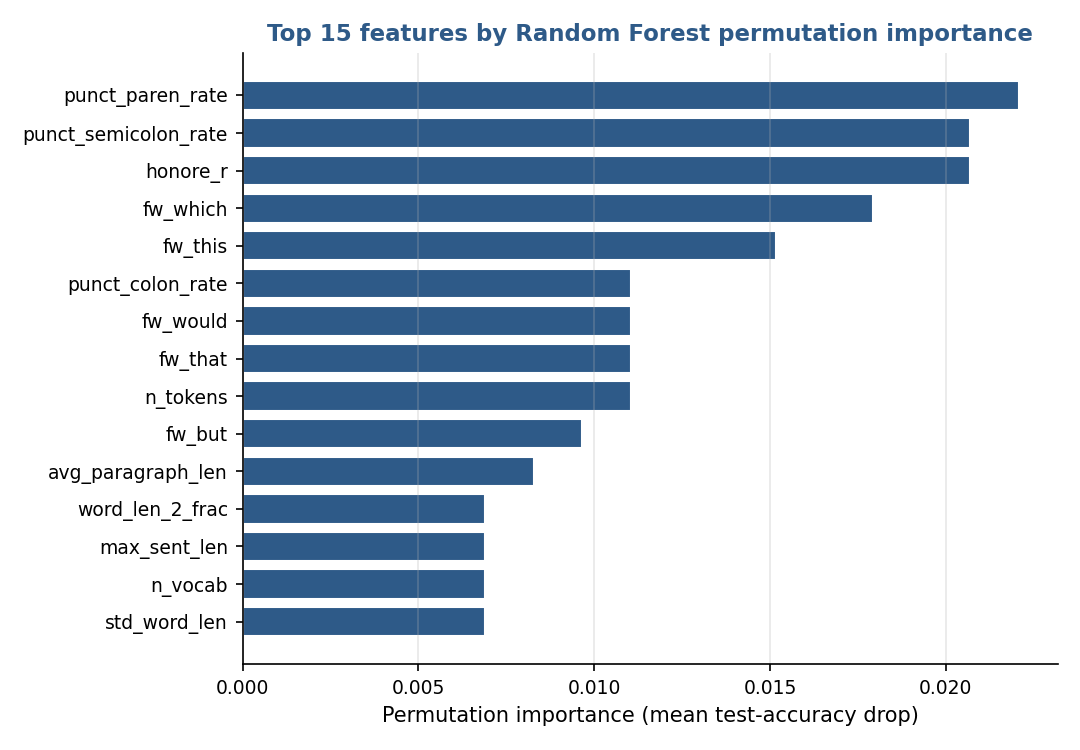
\includegraphics[width=0.72\linewidth]{../src/neural_network/outputs/rf_permutation_importance.png}
  \caption{The $15$ most informative features by Random Forest permutation
  importance (mean drop in held-out accuracy when a feature is shuffled).
  Punctuation habits (parenthesis, semicolon, colon rates), a vocabulary-richness
  measure (Honor\'e's $R$), and a handful of function words (\code{which},
  \code{this}, \code{would}, \code{that}) dominate --- exactly the
  topic-independent, stylistic signals we want.}
  \label{fig:featimp}
\end{figure}

\begin{keybox}
\keytitle{Why early stopping?}
With only $\sim 520$ training articles and thousands of weights, an NN can
memorise the training set. We pass \code{early\_stopping=True}: \code{sklearn}
holds out $10\%$ of the training data as an internal validation set and halts
when its score fails to improve for \code{n\_iter\_no\_change=15} consecutive
epochs (\code{batch\_size=32}, \code{max\_iter=500}). This curbs over-fitting
and makes the depth comparison fair --- every architecture is trained under
the same stopping rule.
\end{keybox}

\subsection{Model Selection and Results}

Figure~\ref{fig:validation} shows validation accuracy for every
feature-subset $\times$ depth combination. The clear winner is \textbf{all
$107$ features with a single hidden layer} (validation accuracy $0.943$).
Two patterns already stand out: using all $107$ features never hurts, and the
deepest network ($50$ layers) collapses to chance --- a phenomenon we return
to in Section~\ref{ssec:depth}.

\begin{figure}[H]
  \centering
  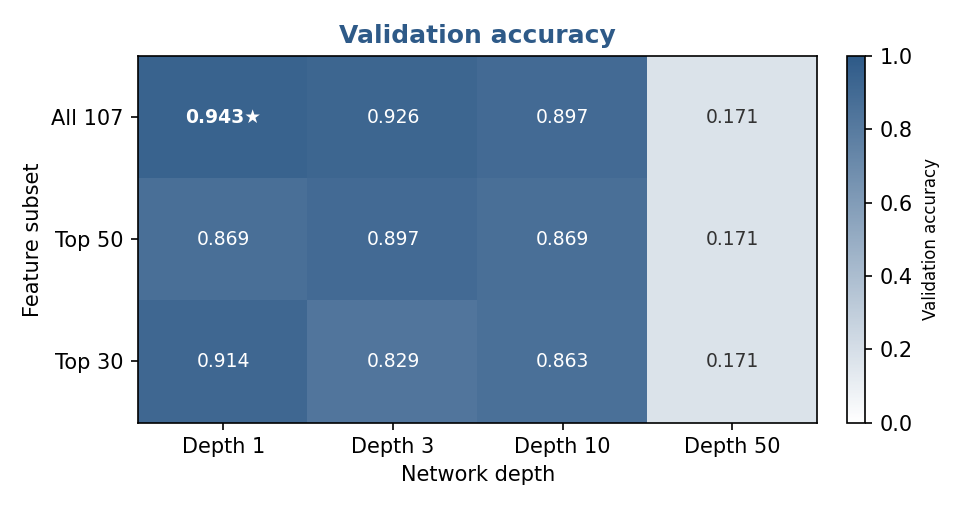
\includegraphics[width=0.78\linewidth]{../src/neural_network/outputs/validation_selection.png}
  \caption{Validation accuracy across feature subsets (rows) and network
  depths (columns). The starred cell --- all $107$ features, depth $1$ --- is
  the selected model. Depth $50$ sits at $0.171$, barely above the six-class
  random baseline of $1/6 \approx 0.167$.}
  \label{fig:validation}
\end{figure}

Retrained on train$+$validation ($698$ articles) and evaluated on the $175$
test articles, the selected model attains the scores in
Table~\ref{tab:nn_test}.

\begin{table}[H]
\centering
\caption{Test-set performance of the selected NN (all $107$ features,
depth $1$).}
\label{tab:nn_test}
\begin{tabular}{lc}
\toprule
\textbf{Metric} & \textbf{Value} \\
\midrule
Accuracy    & $0.949$ \\
Weighted F1 & $0.949$ \\
\bottomrule
\end{tabular}
\end{table}

The confusion matrix (Figure~\ref{fig:cm}) shows a strong diagonal. The
striking result is the \code{none\_of\_the\_5\_authors} class itself:
\textbf{precision, recall, and F1 are all $1.00$}. Not a single unknown-author
article is misattributed to one of the five, and not a single known-author
article is dumped into the ``none'' bin --- the $15$ unknown authors, pooled
together, occupy a region of style-space cleanly separable from the five
targets. Among the five known authors the few errors concentrate on
\code{Raemon} (recall $0.88$) and \code{Scott Alexander} (recall $0.90$),
whose articles are occasionally confused with one another or with
\code{Yudkowsky}; \code{Zvi} is recovered almost perfectly.

\begin{figure}[H]
  \centering
  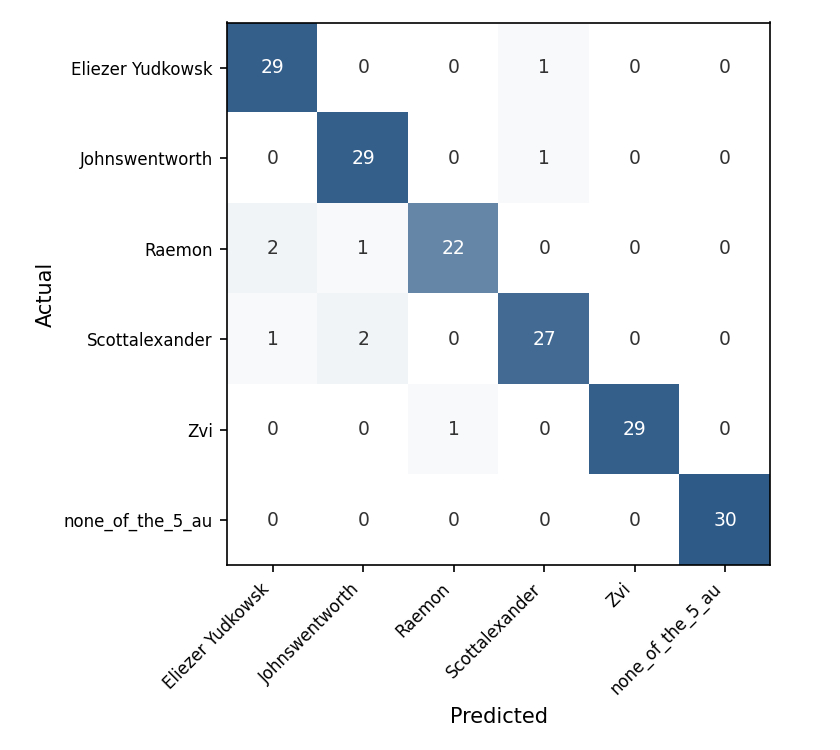
\includegraphics[width=0.56\linewidth]{../src/neural_network/outputs/confusion.png}
  \caption{Test-set confusion matrix (rows $=$ actual, columns $=$
  predicted). The \code{none} row and column are perfectly isolated.}
  \label{fig:cm}
\end{figure}

\begin{keybox}
\keytitle{Why add a ``none'' class instead of using a confidence threshold?}
We tried the simpler route first: train a five-author model and flag any
prediction below some softmax confidence as ``unknown''. It failed
completely. Unknown-author articles routinely produced \emph{high}-confidence
predictions for one of the five known authors, so a confidence threshold
caught essentially none of them. Giving the network labelled ``none''
examples and letting it learn the boundary directly worked much better ---
perfectly, in fact, on the test set. As a bonus, training against $15$
stylistically diverse ``other'' authors also appears to \emph{sharpen} the
boundaries among the five targets: the model learns not just what each
target author looks like, but what they do \emph{not} look
like.
\end{keybox}

\subsection{How Deep Should the Network Be?}
\label{ssec:depth}

A natural instinct is that deeper networks are more powerful, so they should
classify better. Our grid search says otherwise. Figure~\ref{fig:depth} plots
validation accuracy against depth for each feature subset.

\begin{figure}[H]
  \centering
  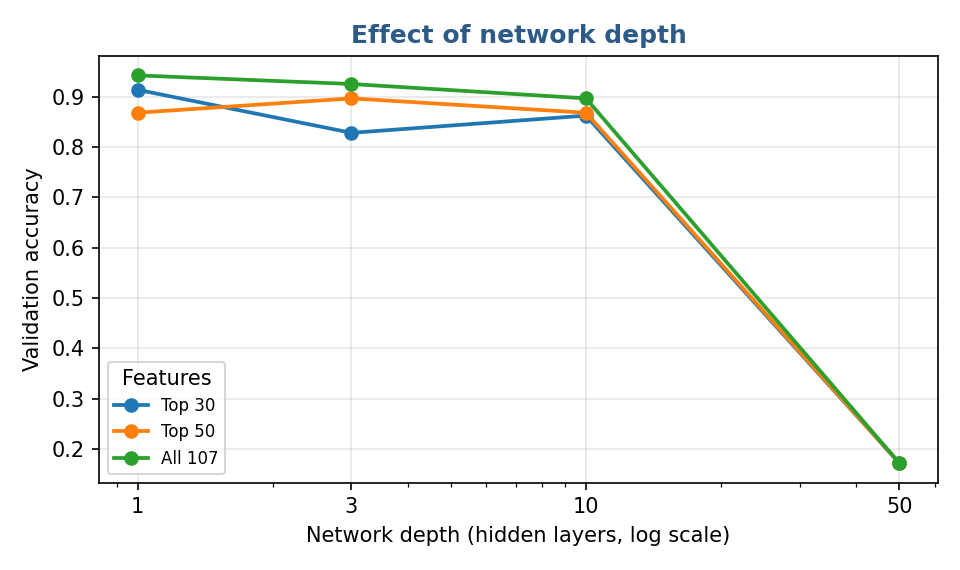
\includegraphics[width=0.7\linewidth]{../src/neural_network/outputs/depth_effect.png}
  \caption{Validation accuracy vs.\ network depth (number of $64$-unit hidden
  layers, log scale). Performance is flat-to-slightly-declining from depth $1$
  to depth $10$, then \textbf{collapses to chance at depth $50$}.}
  \label{fig:depth}
\end{figure}

From depth $1$ to depth $10$ accuracy barely moves --- the extra layers buy
nothing because the decision boundaries between these classes are already
well within reach of a shallow network on $107$ informative features. At
depth $50$ every configuration collapses: validation accuracy falls to
$0.171$, essentially the random baseline of $1/6\approx 0.167$. The network
has stopped learning anything.

\begin{keybox}
\keytitle{Why the deep network fails}
This is not over-fitting --- an over-fit network would still score well above
chance on validation. It is an \emph{optimisation} failure. Stacking $50$
plain fully-connected ReLU layers with no residual connections or
normalisation produces vanishing gradients: the error signal is attenuated
layer by layer during backpropagation, so the early layers receive almost no
useful gradient. Combined with early stopping on a small dataset, training
halts before the network escapes its near-random initialisation. The lesson
is concrete: for tabular stylometric features, \textbf{a shallow NN is not
just sufficient but preferable}.
\end{keybox}

\paragraph{Are the gradients actually vanishing?}
The vanishing-gradient explanation is testable, so we test it. We
re-implement the same architecture in numpy --- Glorot-uniform initialisation
with bound $\sqrt{6/(\text{fan\_in}+\text{fan\_out})}$ (exactly what
\code{sklearn} uses for ReLU layers), ReLU hidden units, softmax output,
cross-entropy loss --- and read off the gradient of the loss with respect to
every layer's weights from a single forward/backward pass on the standardised
features. Averaging over $50$ random initialisations,
Figure~\ref{fig:grad} reports the root-mean-square (RMS) of the weight
gradients at each layer, at the moment training begins.

\begin{figure}[H]
  \centering
  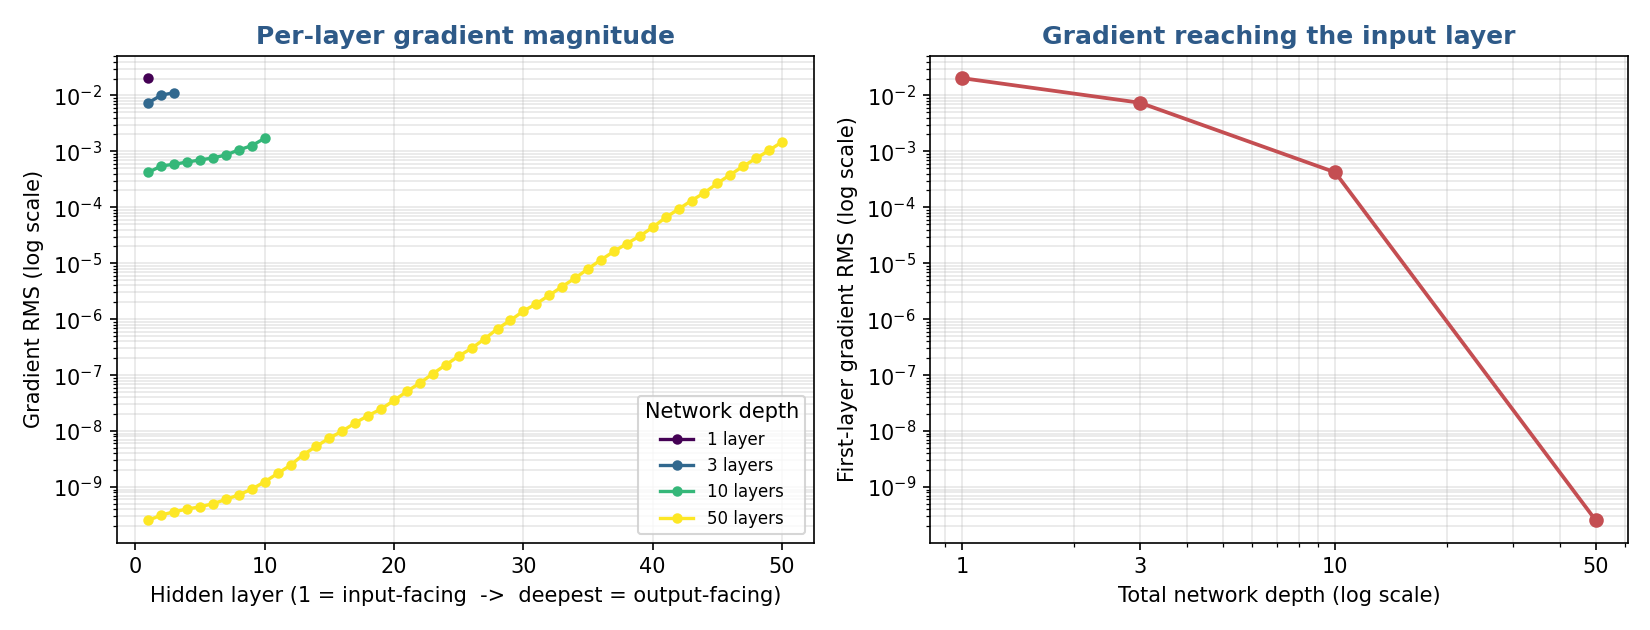
\includegraphics[width=0.95\linewidth]{../src/neural_network/outputs/gradient_health.png}
  \caption{Gradient health at initialisation. \textit{Left}: RMS weight
  gradient per layer, from the input-facing layer ($1$) to the output-facing
  layer, one curve per depth (log scale). \textit{Right}: the gradient
  reaching the input-facing first layer as a function of total depth. Both
  axes are logarithmic.}
  \label{fig:grad}
\end{figure}

The signature is unmistakable. In the shallow networks the gradient is
roughly uniform across layers --- at depth $1$ the input layer already sees
an RMS gradient of $2.0\times10^{-2}$, only $3.5\times$ smaller than the
output layer. As depth grows the gradient decays geometrically on its way
back to the input, so the first layer is starved
(Table~\ref{tab:grad}). By $50$ layers the input-facing layer receives an
RMS gradient of $2.5\times10^{-10}$ --- eight orders of magnitude weaker than
in the shallow net, and $2\times10^{7}$ times weaker than the output layer of
the \emph{same} network.

\begin{table}[H]
\centering
\caption{RMS weight gradient at initialisation, averaged over $50$ inits.
The first layer (input-facing) is the one that must learn feature
combinations; its gradient collapses with depth.}
\label{tab:grad}
\begin{tabular}{rccc}
\toprule
\textbf{Depth} & \textbf{First-layer grad} & \textbf{Output grad}
    & \textbf{Ratio (out\,/\,first)} \\
\midrule
$1$  & $2.0\times10^{-2}$  & $7.0\times10^{-2}$ & $3.5$ \\
$3$  & $7.4\times10^{-3}$  & $3.1\times10^{-2}$ & $4.2$ \\
$10$ & $4.2\times10^{-4}$  & $5.8\times10^{-3}$ & $13.7$ \\
$50$ & $2.5\times10^{-10}$ & $5.5\times10^{-3}$ & $2.2\times10^{7}$ \\
\bottomrule
\end{tabular}
\end{table}

A weight that sees a gradient of $10^{-10}$ cannot move: with early stopping
monitoring a validation score that never improves, training halts within a
few epochs and the deep network never leaves its random initialisation ---
which is exactly the chance-level accuracy we saw at depth $50$. This
confirms the collapse is an \emph{optimisation} pathology, not a capacity or
over-fitting one. The standard fixes (residual connections, batch/layer
normalisation, He initialisation) all exist precisely to keep this gradient
alive; none are warranted here, because the shallow network already solves
the task.

% =============================================================================
\section{Conclusion}
\label{sec:conclusion}

Six things stand out when we compare the experiments against each other:

\begin{itemize}\setlength\itemsep{4pt}
  \item \textbf{Article length matters much more than the number of
        articles per author.} As $N$ grew from $100$ to $1{,}500$ words,
        ARI jumped from $0.07$ to $0.48$ --- almost a $7\times$ change.
        The $M$-sweep showed a much smaller gain on both corpora we
        tried: on \texttt{cleaned\_10}, ARI moved from $0.42$ at $M{=}5$
        to $0.55$ at $M{=}20$ (still climbing, but slowly), and on the
        \texttt{sup\_4} subset --- four specific authors with $76$--$79$
        articles each, the only group where we could push $M$ much
        further --- ARI moved from $0.34$ to $0.46$ between $M{=}5$ and
        $M{=}25$ and then flattened to $\sim\!0.46$ through $M{=}40$.
        The plateau is specific to those four authors and might not hold
        more generally, but the broader pattern is clear: extra length
        keeps helping over a wide range, while extra articles only help
        in small amounts. If we want better clustering, longer articles
        are the first thing to chase; more posts per author come second.

  \item \textbf{A person's writing style changes noticeably over a few
        years.} Same authors, same features, same pipeline --- yet ARI
        fell from $0.66$ on pre-$2022$ posts to $0.53$ on post-$2024$
        posts. The gap is too large to be noise. We can't tell whether
        the cause is AI polishing, topic shift, or just normal change,
        but the lesson is the same: writing style is not a fixed thing
        we can pin down once and reuse forever.

  \item \textbf{How you compare two articles matters more than which
        classifier you use.} Logistic regression scored within about
        $1$ percentage point of the RBF-SVM on every metric --- accuracy,
        F1, ROC-AUC --- even though the two models draw very different
        decision boundaries. The thing that did the real work was the
        pair encoding ($|f_1{-}f_2|$, $(f_1{-}f_2)^2$, $f_1 \odot f_2$):
        once two articles are turned into those three combinations, the
        problem is already almost linear. The first question for this
        kind of task isn't ``which model?''; it's ``what do I feed it?''.

  \item \textbf{The verifier worked on authors it had never seen.}
        We trained the SVM on $28$ authors and tested it on $7$
        completely different ones, and it still reached ROC-AUC
        $\approx 0.81$. That means the model learned a general
        ``same-author vs.\ different-author'' rule, not just the
        fingerprints of the people it was trained on --- and that is
        why this kind of verifier can be used in the wild, where the
        candidates won't be in the training set.

  \item \textbf{If the model might see an unknown author, give it
        labelled unknowns to train on.} Trying to flag unknown articles
        by looking for low softmax confidence on a $5$-class model
        \emph{failed}: unknowns produced confidently wrong answers, not
        low-confidence ones. Adding an explicit ``none of the $5$
        authors'' class --- built from $15$ other LessWrong writers ---
        gave perfect rejection (P, R, F1 all $1.00$). The model can
        recognise outsiders, but only after we have shown it what an
        outsider looks like.

  \item \textbf{Deeper neural networks did not help here, and very deep
        ones broke.} Validation accuracy was essentially the same from
        $1$ layer through $10$ layers, and then dropped to random
        guessing ($0.171$) at $50$ layers. The gradient check explained
        why: by depth $50$ the gradient reaching the first layer was
        $\sim 2.5 \times 10^{-10}$, so the network could not actually
        train. On only $873$ examples in $107$ dimensions, a single
        hidden layer is already enough --- more layers just add risk
        without adding accuracy.
\end{itemize}

\end{document}
